\documentclass[a4paper,12pt]{article}

%\documentclass[draft, 12pt]{article}
% ================================================== DATOS ==================================================

% Información de la materia
\newcommand{\codMateria}{TA138}
\newcommand{\nombreMateria}{Taller de Diseño de}
\newcommand{\cuatrimestre}{1.\textsuperscript{er} Cuatrimestre}

% Información del TP
\newcommand{\TpTitulo}{Proyecto Integrador -- Checkpoint 5}
\newcommand{\fecha}{\today}
\newcommand{\group}{Grupo 5}

% Información de alumnos
\newcommand{\nombreA}{Lautaro García Vitale}
\newcommand{\padronA}{110.028}
\newcommand{\emailA}{lagarciav@fi.uba.ar}

\newcommand{\nombreB}{Santiago Manuel Cabrera}
\newcommand{\padronB}{110.445}
\newcommand{\emailB}{smcabrera@fi.uba.ar}

\newcommand{\nombreC}{Francisco Javier Moya}
\newcommand{\padronC}{109.899}
\newcommand{\emailC}{fjmoya@fi.uba.ar}

% ================================================== PAQUETES =================================================

% Codificación y lenguaje
\usepackage[utf8]{inputenc}
\usepackage{siunitx}
\usepackage[ddmmyy]{datetime}
\usepackage[language=spanish]{lipsum}
\usepackage[spanish]{datetime2}
\usepackage[T1]{fontenc}
\usepackage[spanish,es-nodecimaldot]{babel}

% -------- CAMBIAR "CUADRO" POR "TABLA" --------
\addto\captionsspanish{
    \renewcommand{\tablename}{Tabla}
}

\usepackage[a4paper,margin=2.5cm]{geometry}
\usepackage{amsmath,amssymb,amsthm,mathtools}
\usepackage{bm}
\usepackage{setspace}
\usepackage{hyperref}
\usepackage{enumitem}

% Márgenes y página
\usepackage{geometry}
\usepackage{fancyhdr}
\usepackage{emptypage}
%\usepackage{parskip}

% Encabezado personalizado
\pagestyle{fancy}
\fancyhf{}
\rhead{\group}
\lhead{\TpTitulo}
\cfoot{\thepage}
\setlength{\headheight}{14.5pt}

% Tipografía matemática
\usepackage{mathtools}
\usepackage{amssymb}
\usepackage{amsfonts}
\usepackage{amsthm}
\usepackage{yhmath}
\usepackage{dsfont}
\usepackage{esdiff}
\usepackage{xfrac}
\usepackage{upgreek}
\usepackage{siunitx}
\sisetup{output-decimal-marker = {,}} % Configura la coma como separador
\sisetup{per-mode=reciprocal, separate-uncertainty=true}

% Gráficos y tablas
\usepackage{graphicx}
\usepackage{float}
\usepackage{booktabs}
\usepackage{caption}
\usepackage{subcaption}
\usepackage{multirow}
\usepackage{adjustbox}
\usepackage{hyperref}

% TikZ y gráficos avanzados
\usepackage{pgfplots}
\pgfplotsset{compat=1.18}
\usepackage{tikz}

% Código fuente y resaltado
\usepackage{minted}
\usepackage{tcolorbox}
\definecolor{codebg}{rgb}{0.95,0.95,0.95}  % Color de fondo del código
\usemintedstyle{friendly}                  % Estilo del resaltado de sintaxis
\setminted{
    linenos=true,                          % Numeración de líneas
    bgcolor=codebg,                        % Color de fondo del código
    fontsize=\footnotesize,                % Tamaño de la fuente
    frame=lines,                           % Estilo del marco
    framesep=2mm,                          % Separación del marco
    baselinestretch=1.2,                   % Espaciado entre líneas
    breaklines=true,                       % Romper líneas largas automáticamente
    encoding=utf8,                         % Codificación del archivo
    tabsize=4,                             % Tamaño de la tabulación
}

% Misceláneo
\usepackage{anyfontsize}
\usepackage{xcolor}
\usepackage{url}
\usepackage{comment}
\usepackage{multicol}
\usepackage[numbers,square]{natbib}

% Estilo de bibliografía
\bibliographystyle{IEEEtran}

% ==============================================================================================================
% ==============================================================================================================

\begin{document}

% ================================================== CARÁTULA ==================================================

\pagenumbering{arabic} % Comienza la numeración

\vspace{-1 cm} % La primera hoja tiene que tener menos espaciado

\begin{center}
  \begin{minipage}{0.8 cm}
    
\includegraphics[width=\linewidth]{img/fiuba.png}
  \end{minipage}
  \begin{minipage}{\widthof{\large{\textsc{Universidad de Buenos Aires}}}}
    \centering
    \large{\textsc{Universidad de Buenos Aires}}\\
    \large{\textsc{Facultad de Ingeniería}}\\
    \small{Año 2026 -- \cuatrimestre}
  \end{minipage}
\end{center}
\vspace{10mm}
\begin{center}
  \huge{\underline{\textsc{\nombreMateria}}} \\
  \huge{\underline{\textsc{Circuitos Electrónicos}}} \\
  \vspace{7 pt}
  \Large{\TpTitulo \\}
  \vspace{3mm}
  \large{\group}
\end{center}

\newcommand{\anchopadron}{\widthof{000 000}}
\begin{center}
  \begin{tabular}{l l l}
    \nombreA & \parbox{\anchopadron}{\raggedleft \padronA} & \texttt{\emailA} \\
    \nombreB & \parbox{\anchopadron}{\raggedleft \padronB} & \texttt{\emailB} \\
    \nombreC & \parbox{\anchopadron}{\raggedleft \padronC} & \texttt{\emailC} 
  \end{tabular}
\end{center}
\vspace{8mm}

\begin{center}
\renewcommand{\arraystretch}{1.3}
\begin{tabular}{@{}r p{0.62\textwidth}@{}}
\textbf{Tutor:} & Ing. Federico Gabriel D'Angiolo. \\ 
\textbf{Docentes:} & Ing.Julio Guillermo Zola, Ing. Marcelo Adrián Bruno, Ing. Sergio Quinteros e Ing. Juan Guido Salaya.
\end{tabular}
\end{center}

\vspace{2em}
\thispagestyle{empty}

\begin{abstract}
En este informe se presenta el diseño, implementación y validación experimental de una fuente conmutada tipo \textit{buck} a lazo cerrado, desarrollada como etapa final del proyecto integrador. Se aborda la caracterización del inductor, el ajuste del generador PWM, la selección de componentes de la etapa de potencia, la implementación del \textit{gate driver}, el diseño de la red de compensación y la fabricación del PCB. También se incluyen simulaciones de estabilidad y mediciones sobre el prototipo final, junto con la integración de la etapa reguladora LDO. Los resultados obtenidos verifican un funcionamiento estable de la fuente, con buena regulación de línea y de carga, eficiencias superiores al $90\%$ para $V_{in}=12\,$V en el rango ensayado y un desempeño adecuado frente a variaciones de entrada y carga. A partir de la comparación entre el modelo teórico, las simulaciones y las mediciones experimentales, se identificaron y corrigieron diferencias propias de la implementación práctica, obteniéndose finalmente una fuente funcional, eficiente y experimentalmente validada.
\end{abstract}

\newpage
\tableofcontents
\newpage

\section{Introducción}
El presente informe corresponde al quinto y último \textit{checkpoint} del proyecto integrador, cuyo objetivo fue completar el diseño, la implementación y la validación experimental de una fuente conmutada tipo \textit{buck} operando a lazo cerrado. A diferencia de las entregas anteriores, centradas principalmente en el dimensionamiento teórico y en la verificación parcial de bloques individuales, en esta etapa se integraron todos los subsistemas necesarios para obtener un prototipo funcional.

En primer lugar, se retomó la caracterización del inductor construido, ya que este componente resulta determinante para el comportamiento dinámico del convertidor. A partir de las mediciones realizadas se verificó su inductancia efectiva, su margen frente a la saturación y su compatibilidad con las condiciones de operación previstas para la fuente.

Luego se desarrolló la etapa de potencia y control del convertidor. Esto incluyó la modificación del generador PWM, la selección de los diodos de rueda libre, la incorporación de una carga fantasma, el análisis de los capacitores de entrada y salida, el diseño del \textit{gate driver} y la implementación de una red de compensación para estabilizar el sistema a lazo cerrado. También se presenta el circuito final adoptado y las decisiones de diseño que permitieron adaptar el modelo teórico a una implementación práctica.

Posteriormente, se realizaron simulaciones para validar la respuesta temporal y frecuencial del sistema compensado. Estas permitieron comparar el comportamiento del convertidor antes y después de la compensación, evaluar la estabilidad del lazo y estimar el desempeño esperado frente a variaciones de carga y tensión de entrada.

Finalmente, se diseñó e implementó el PCB del prototipo y se llevaron a cabo mediciones experimentales sobre la fuente construida. En particular, se analizaron las señales del \textit{gate driver}, la conmutación de la etapa de potencia, la eficiencia, la regulación de línea y carga, y el \textit{ripple} de salida. De esta manera, el informe busca contrastar los resultados teóricos y simulados con el comportamiento real del circuito, identificando las principales diferencias observadas y las correcciones realizadas durante la puesta en marcha.

\section{Caracterización del inductor}
% Incluir recálculos del inductor y sus mediciones.
Tal y como se especificó en el \textit{checkpoint} anterior, se escogió en núcleo EE3007 del material CF196 ---una ferrita MnZn para fuentes conmutadas de potencia--- de $A_c = 0,60\,\text{cm}^2$ con un entrehierro de 0,25$\,$mm. Esto implica un recálculo de las espiras necesarias para alcanzar la inductancia deseada de $356,5\,\upmu$H. Recordando que
\[
n = \frac{L \, I_L^{\text{max}}}{B_\text{max} \, A_c} 
\quad \text{y} \quad \ell_g = \frac{\mu_0 \, L \, (I_L^{\text{max}})^2}{B_\text{max}^2 \, A_c}  
\]
se puede deducir que
\[
n = \sqrt{\frac{L \, \ell_g}{\mu_0 \, A_c}} \, ,  
\]
por lo que se necesitarán al menos 35 espiras para alcanzar dicha inductancia. De este modo, se obtiene la relación $I_L^{\text{max}} / B_\text{max} = 5,89 \, \text{A/T}$, lo que implica un campo magnético máximo de 0,27$\,$T para una corriente máxima de 1,6$\,$A; o una corriente máxima de 1,77$\,$A para un campo magnético máximo de 0,30$\,$T.

Asimismo, la hoja de datos del núcleo indica
\[
n^2 \, A_L = L\,
\]
con un factor de inductancia $A_L = 140\,\text{nH}$, lo que sugiere que se necesitarán aproximadamente 51 espiras para alcanzar la inductancia deseada.

A fines prácticos, se generaron 47 espiras con un devanado del tipo AWG\#20.

Para caracterizar el inductor, se utilizó el circuito de la Figura~\ref{fig:circuito_inductor}, con una resistencia $R$ de 0.596$\,\Omega$; una tensión de alimentación $V_\text{in}$ de 9$\,$V; una señal cuadrada de 12.5$\,$V de amplitud, 1$\,$kHz de frecuencia y un \textit{duty cicle} del 1$\,$\% que ingresa al \textit{gate} de un transistor MOSFET; y un diodo en paralelo con el inductor cuya inductancia queremos encontrar.

\begin{figure}[H]
\centering
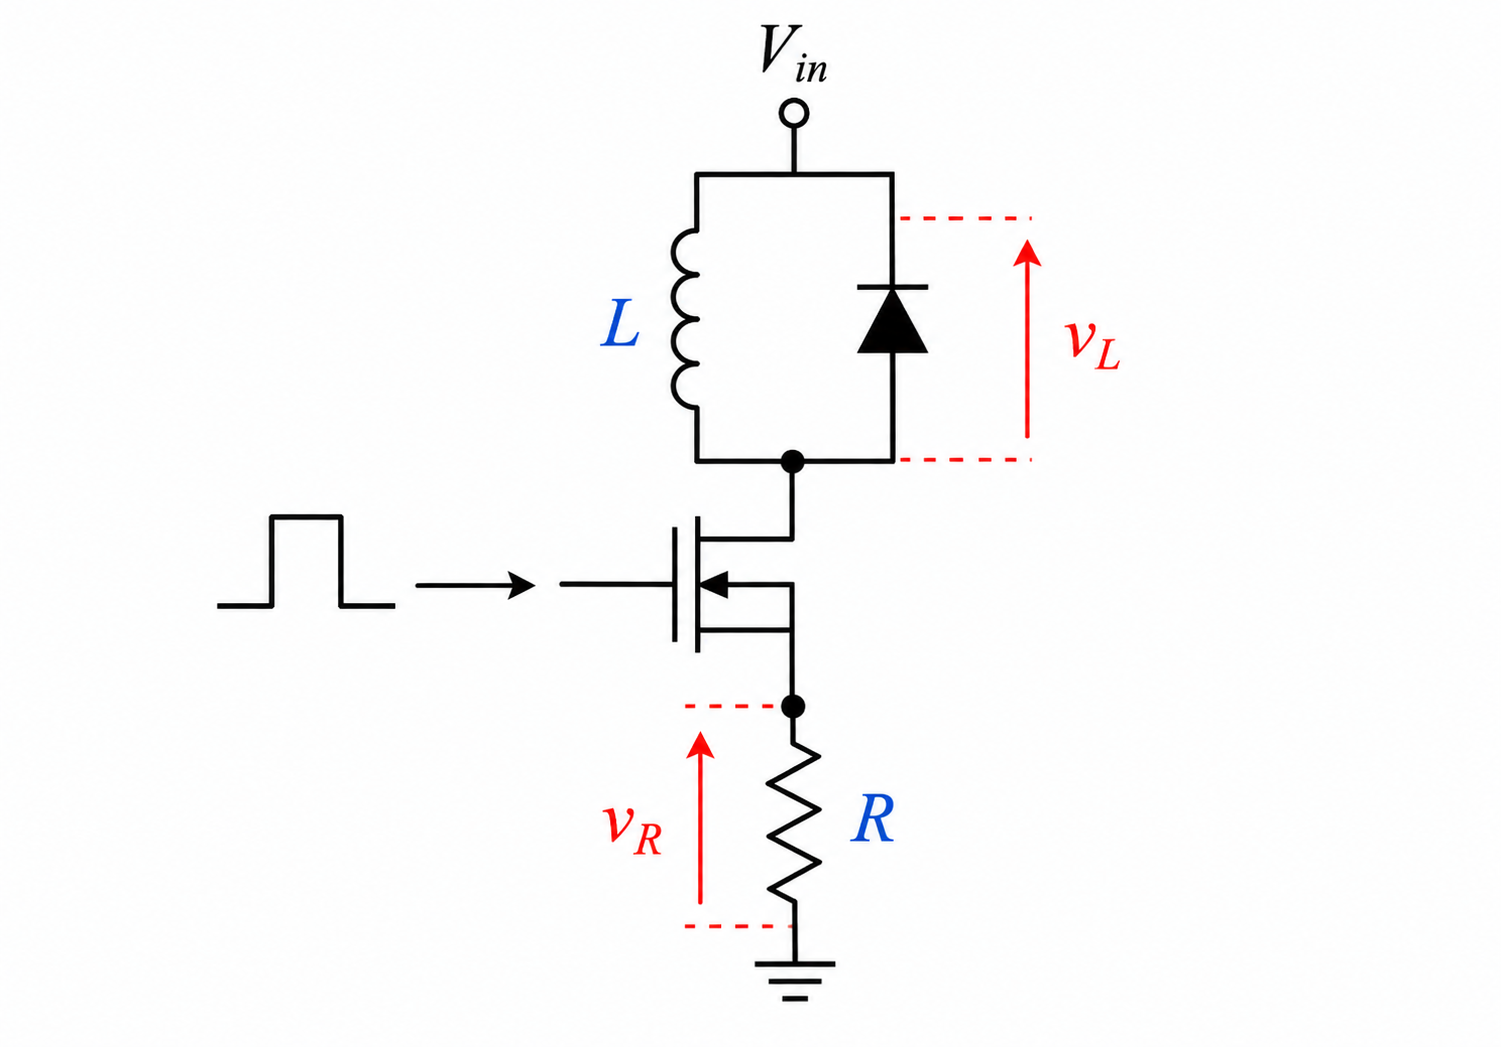
\includegraphics[width = 0.6\textwidth]{img/inductor/circuito_inductor.png}
\caption{Circuito utilizado para caracterizar el inductor.}
\label{fig:circuito_inductor}
\end{figure}

Dado que la resistencia de sensado es pequeña, su corriente ha de ser aproximadamente igual a la corriente que circula por el inductor. La misma, será proporcional a la tensión del resistor:
\[
\Delta i_L = R \, \Delta v_R\,.    
\]

Dado que $v_L = L \cdot \Delta i_L / \Delta t$ y $v_L = V_\text{in} - \Delta v_R$ se obtiene 
\[
L = \frac{V_\text{in} - \Delta v_R}{\Delta i_L / \Delta t} \, .
\]

En la Figura~\ref{fig:lineal} se observa la tensión del resistor, de donde se obtuvo vía cursores $\Delta t = 100\,\upmu$s y $\Delta v_R = 1.1\,$V, por lo que se obtiene una inductancia $L = 408.7\,\upmu$H, un valor superior al diseñado pero aún muy por encima de la inductancia mínima necesaria.

Asimismo, en la Figura~\ref{fig:saturacion} se observa que el inductor llego a la zona de saturación dado el punto de inflexión en la característica a una corriente de saturación $I_S = 4\,$A.

\begin{figure}[H]
\centering
\begin{subfigure}{0.48\textwidth}
\centering
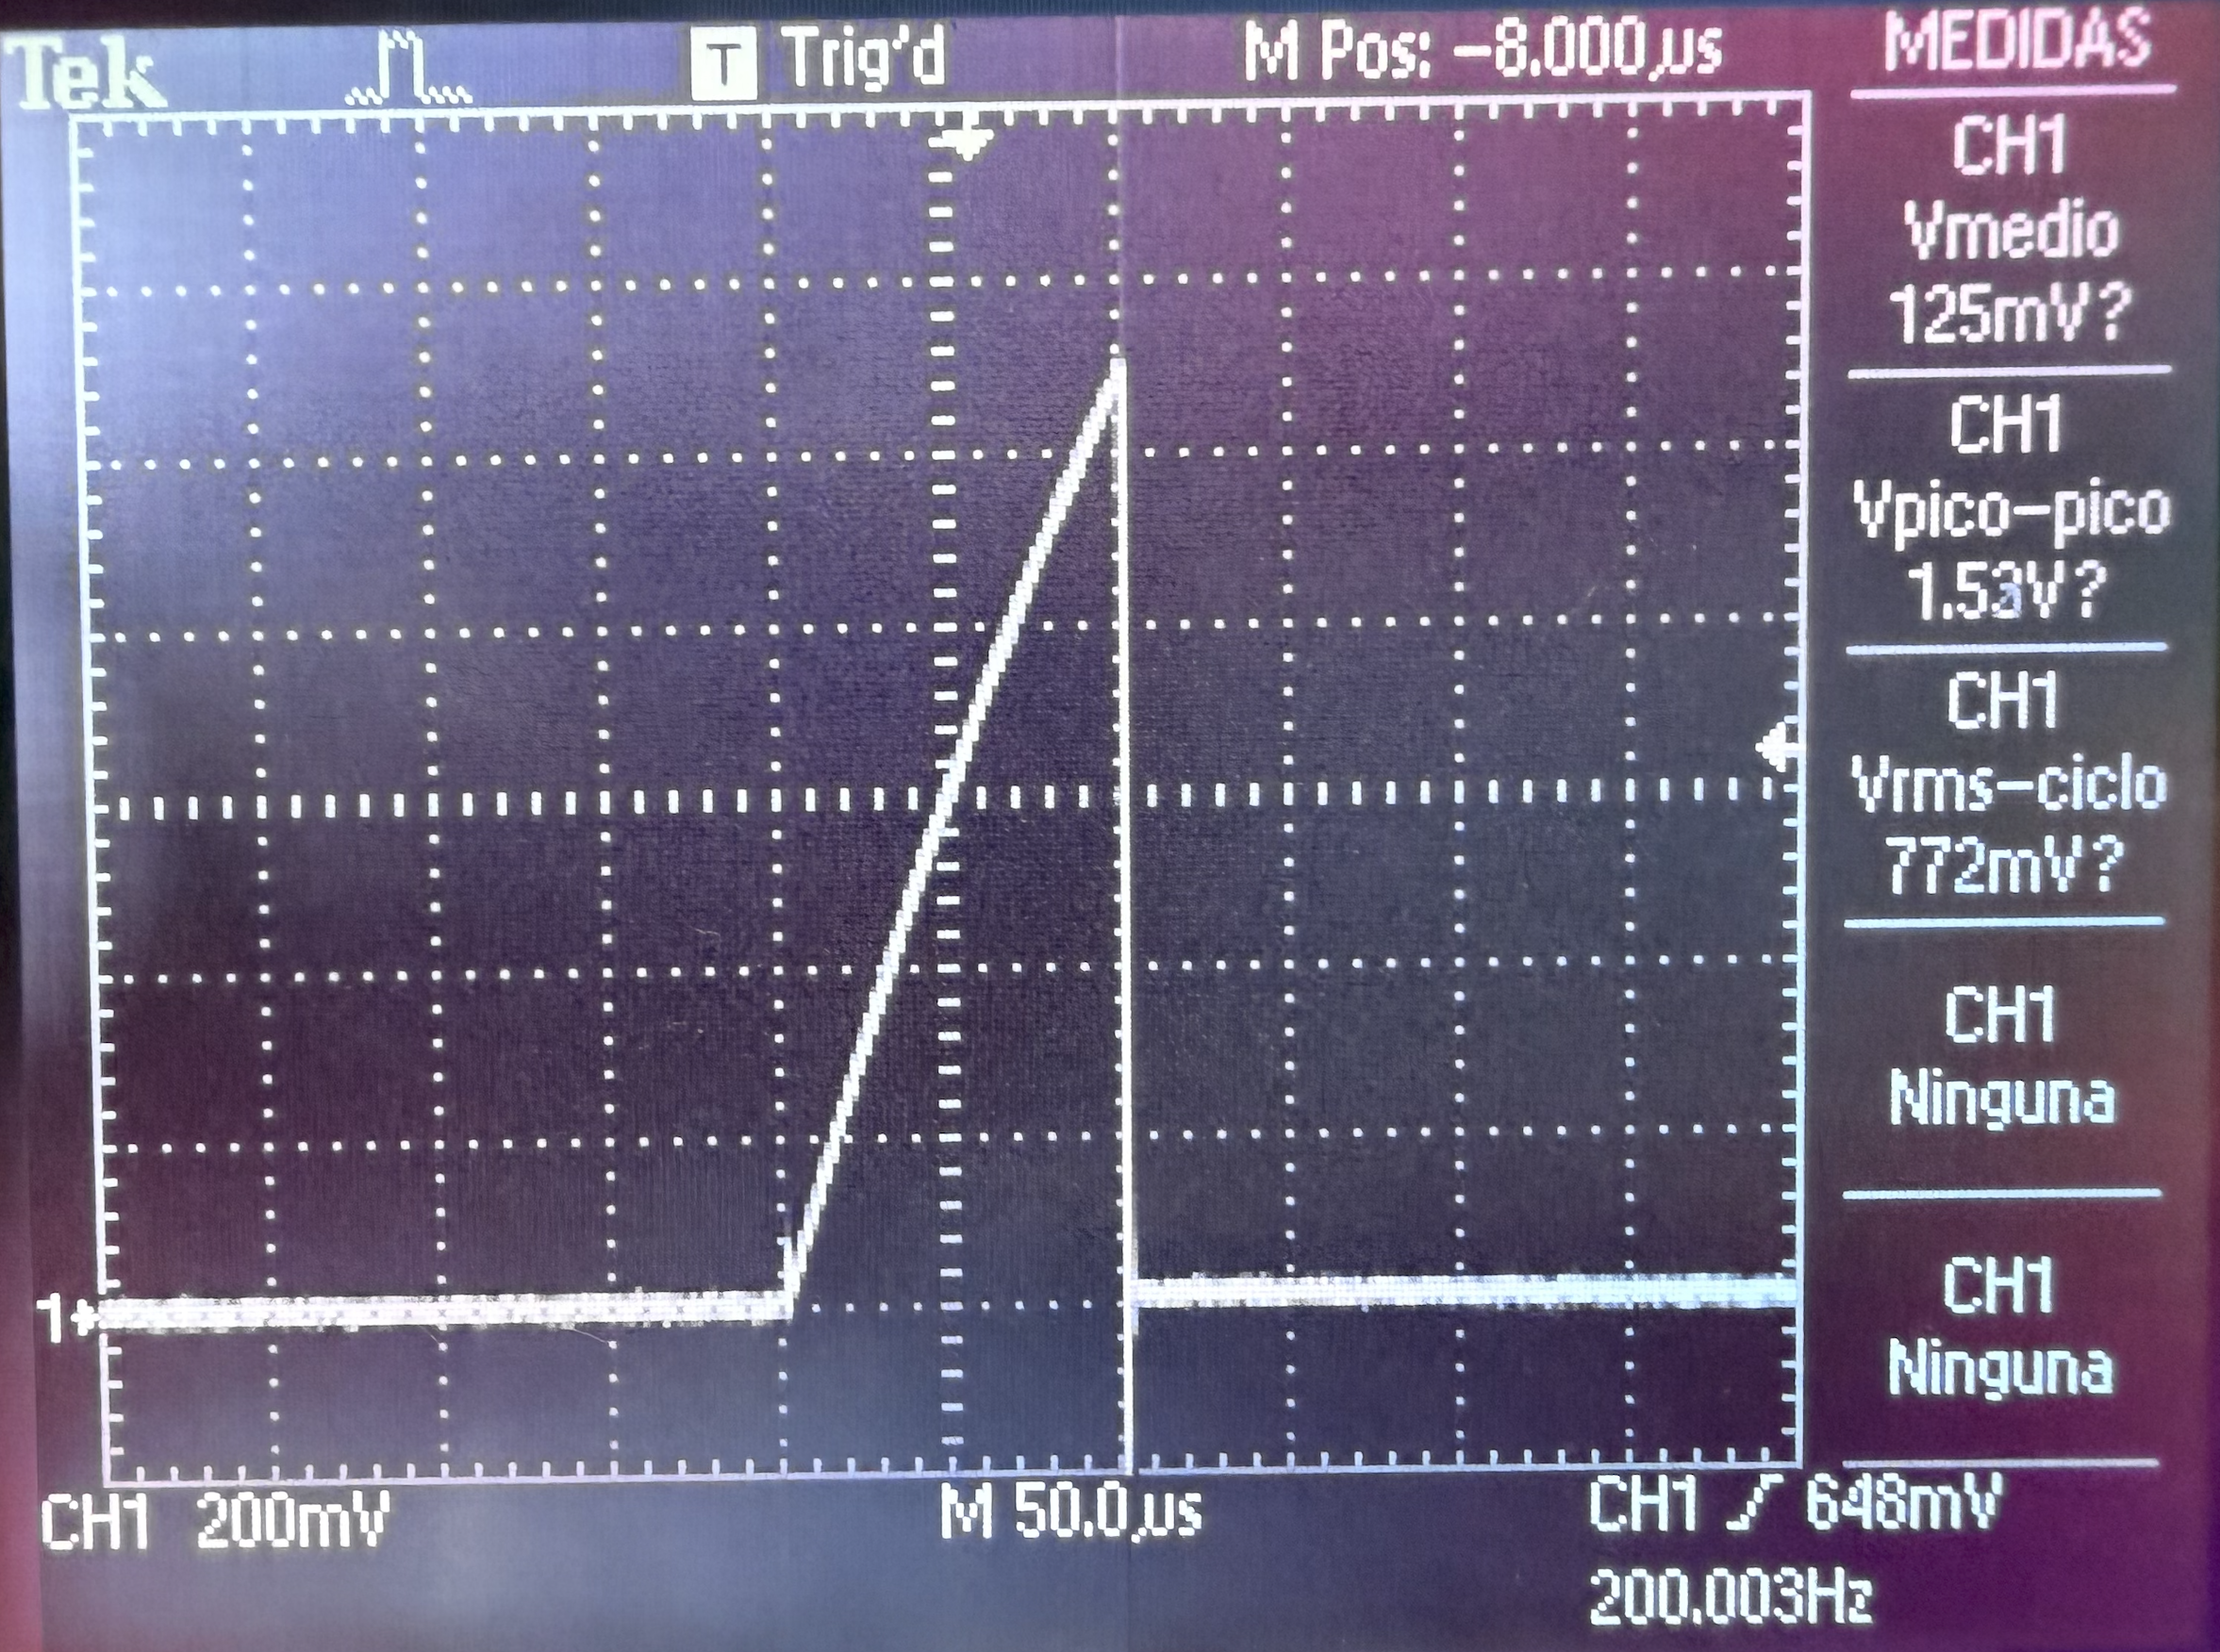
\includegraphics[width=\textwidth]{img/inductor/lineal.png}
\caption{Tensión en el resistor (zona lineal).}
\label{fig:lineal}
\end{subfigure}
\hfill
\begin{subfigure}{0.48\textwidth}
\centering
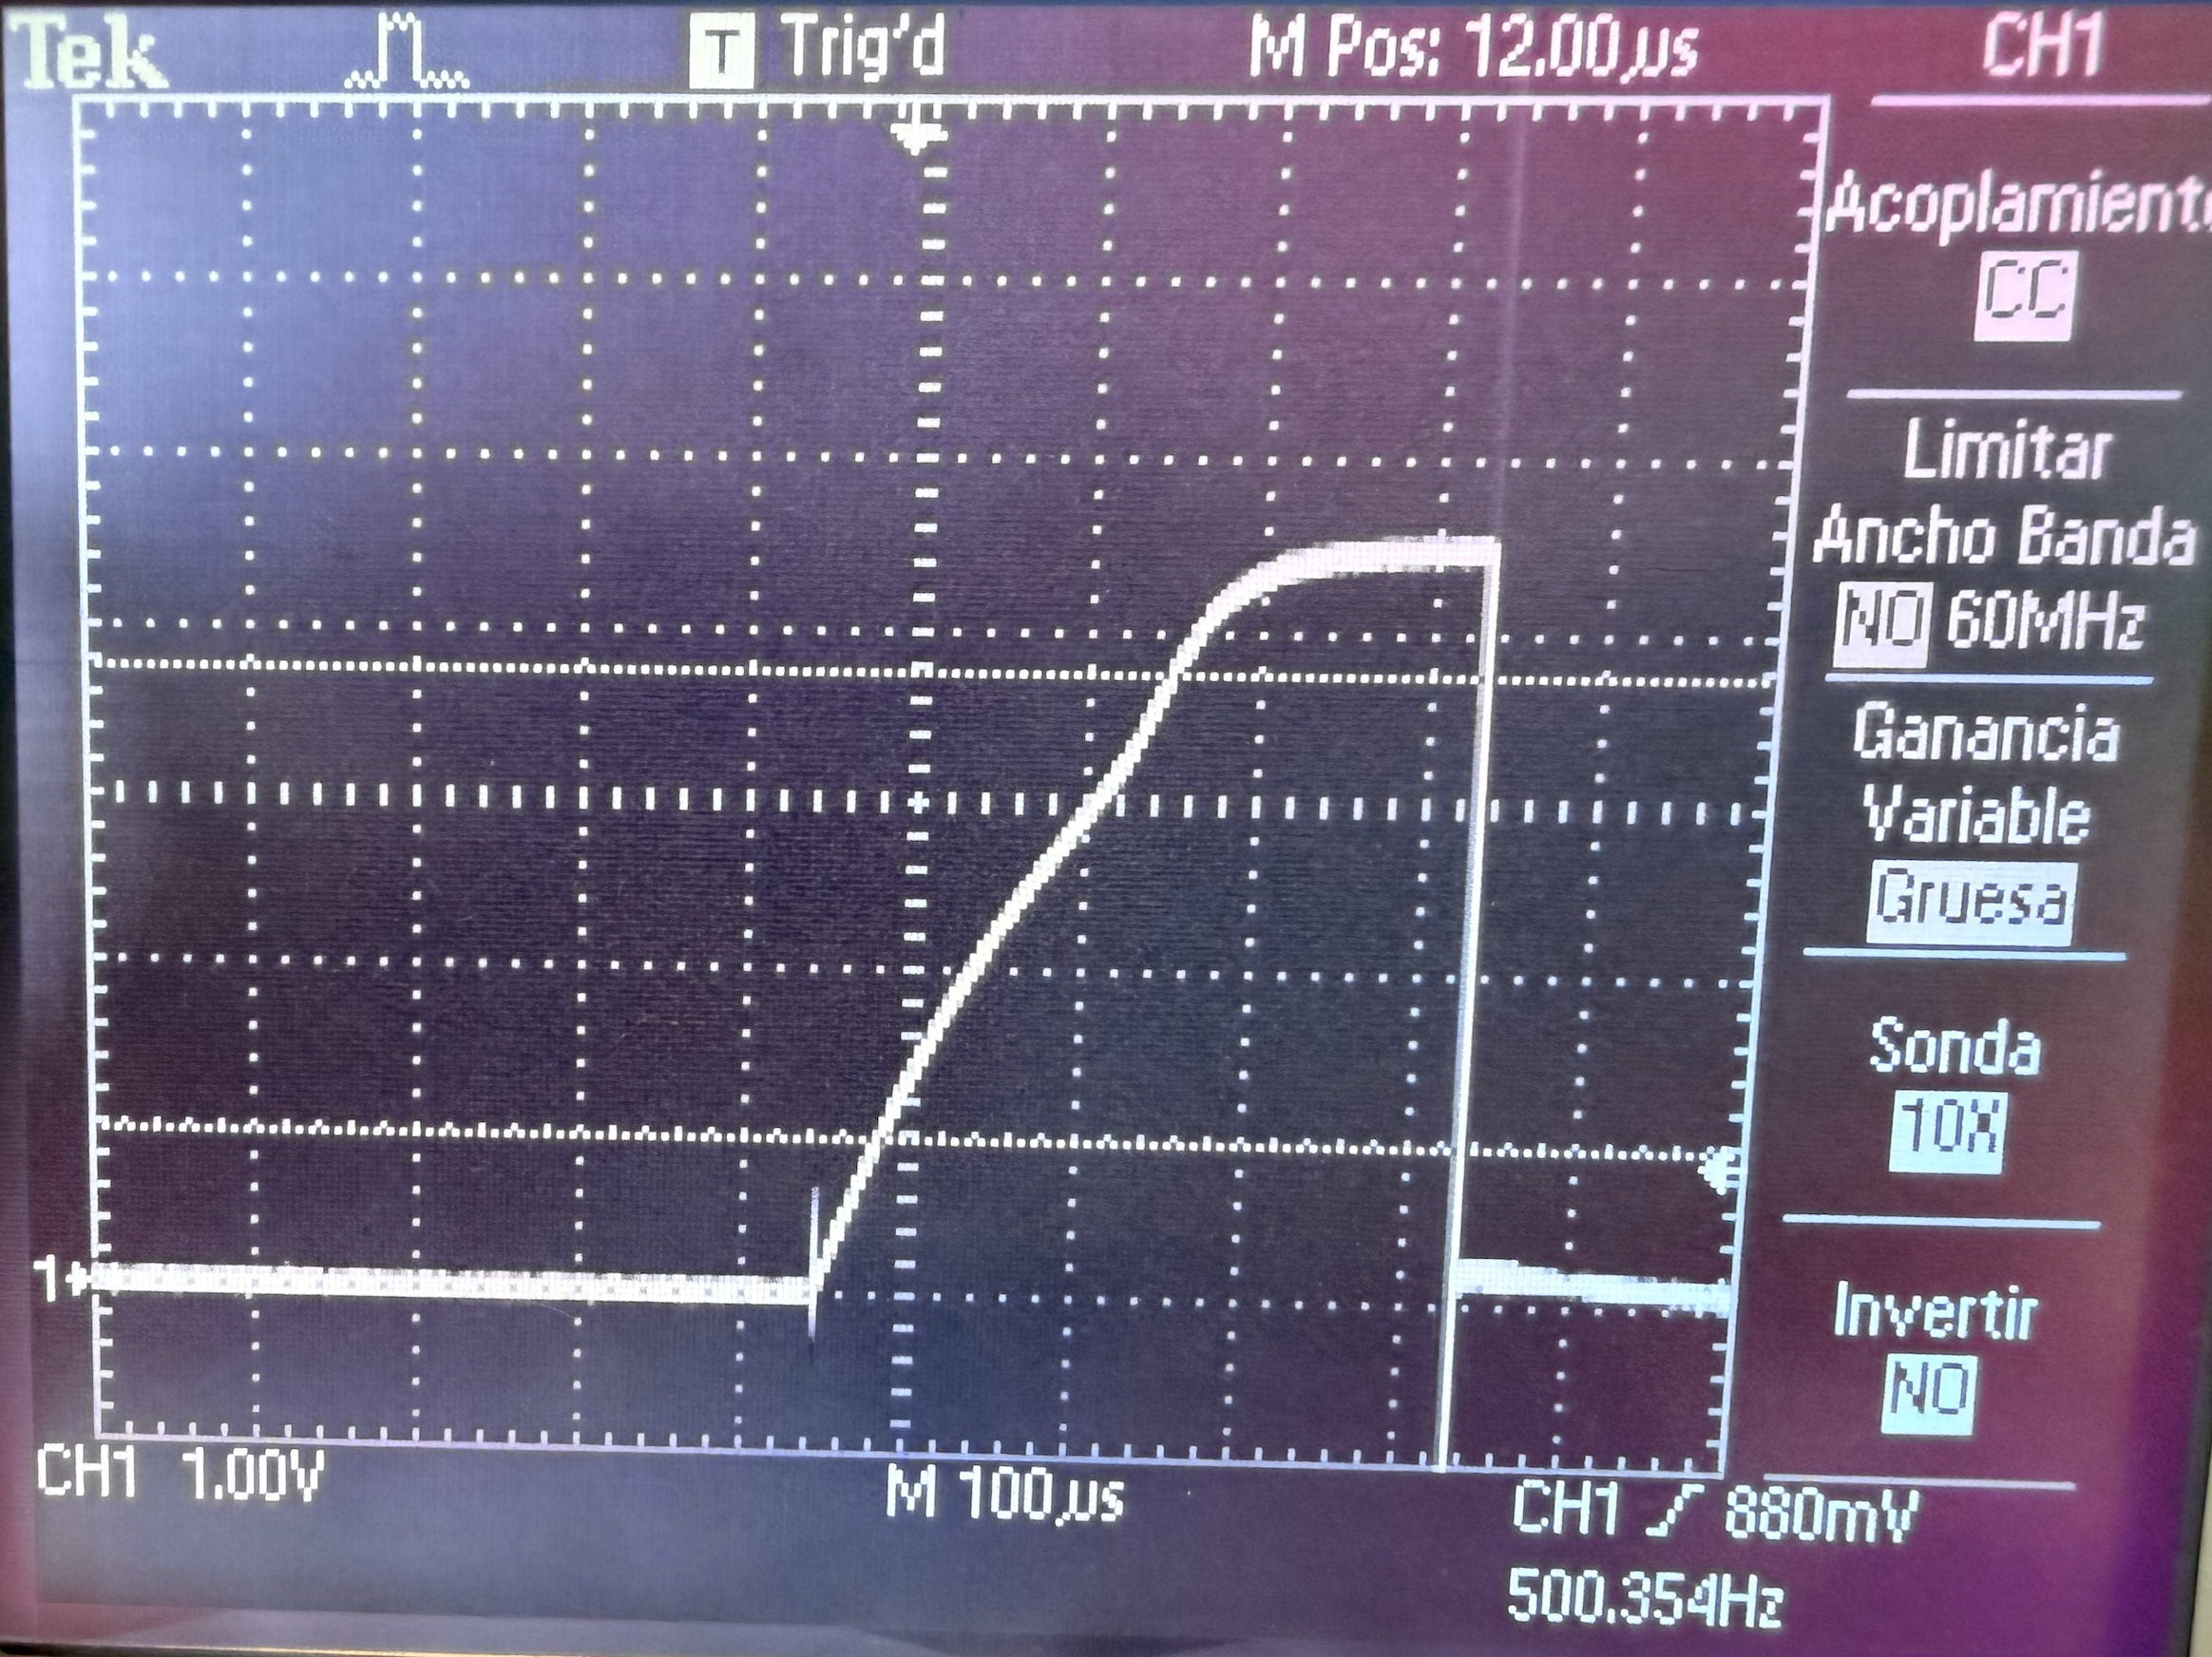
\includegraphics[width=\textwidth]{img/inductor/saturacion.png}
\caption{Tensión en el resistor (saturación).}
\label{fig:saturacion}
\end{subfigure}
\caption{Mediciones utilizadas para caracterizar el inductor.}
\label{fig:mediciones_inductor}
\end{figure}

La densidad de flujo magnético puede estimarse mediante
\[
B = \frac{A_L \, n \, I}{A_c}\,.
\]

Evaluando la expresión para la corriente de saturación se obtiene $B_{\max} = 0.439\ \text{T}\,$. Este resultado concuerda con la curva \(B\)-\(H\) del material CF196 mostrada en la Figura~\ref{fig:campo}, donde puede observarse que la región de saturación comienza aproximadamente para densidades de flujo comprendidas entre \(430\) y \(450\,\text{mT}\). En consecuencia, una corriente de \(4\,\text{A}\) sitúa al núcleo muy próximo al inicio de la saturación magnética, justificando su adopción como corriente máxima de operación.

\begin{figure}[H]
    \centering
    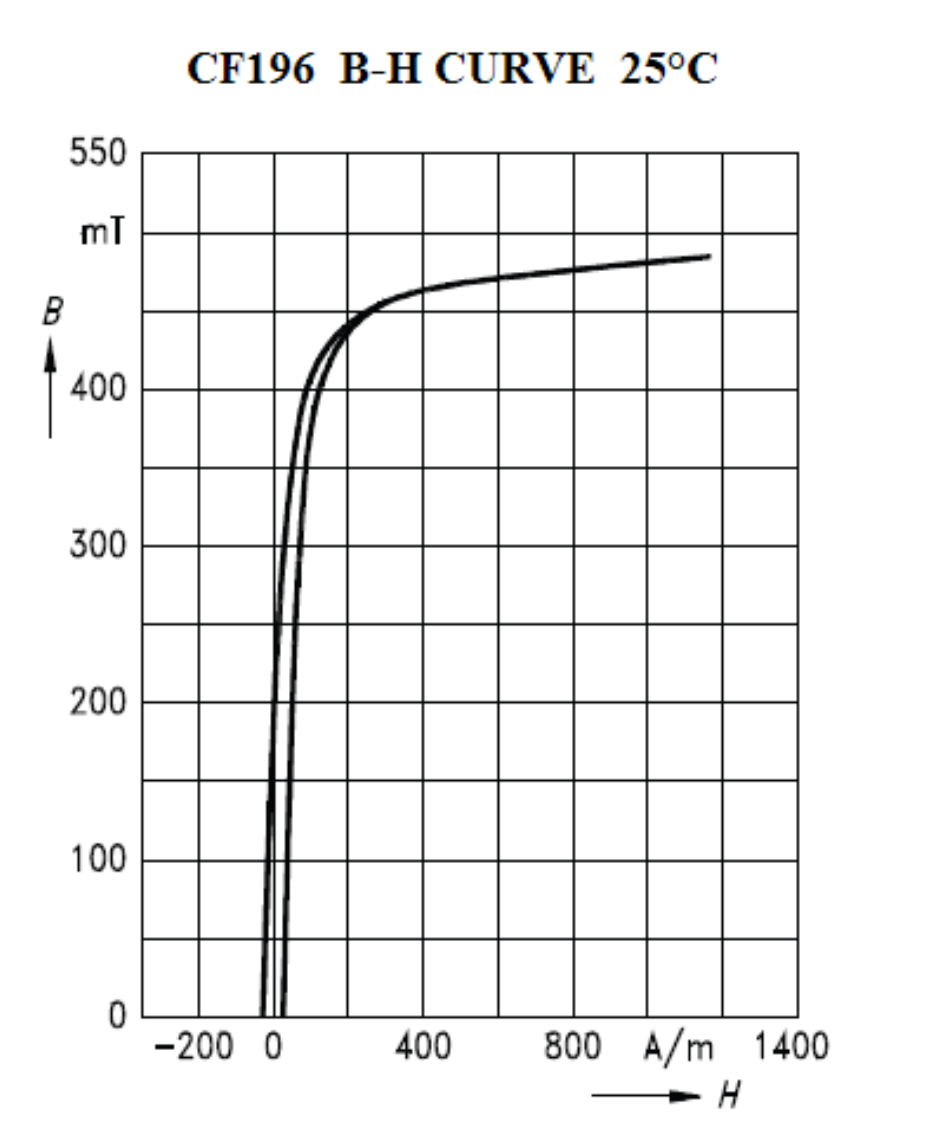
\includegraphics[width = 0.5\textwidth]{img/inductor/campo.png}
    \caption{Curva \(B\)-\(H\) del material CF196 a 25°.}
    \label{fig:campo}
\end{figure}

\section{Diseño de la \textit{buck} a lazo cerrado}
\subsection{Modificación del circuito generador del PWM}

En el desarrollo teórico ideal se supuso que el comparador conmuta instantáneamente
cuando la señal triangular alcanza alguno de los umbrales del disparador Schmitt,
es decir, cuando llega a $V_{IL}$ o a $V_{IH}$ (ver Figura~\ref{fig:comparador-ideal}). Bajo esa hipótesis, el período de oscilación queda determinado únicamente por la pendiente de carga/descarga del
integrador y por la separación entre los umbrales.

\begin{figure}[H]
    \centering
    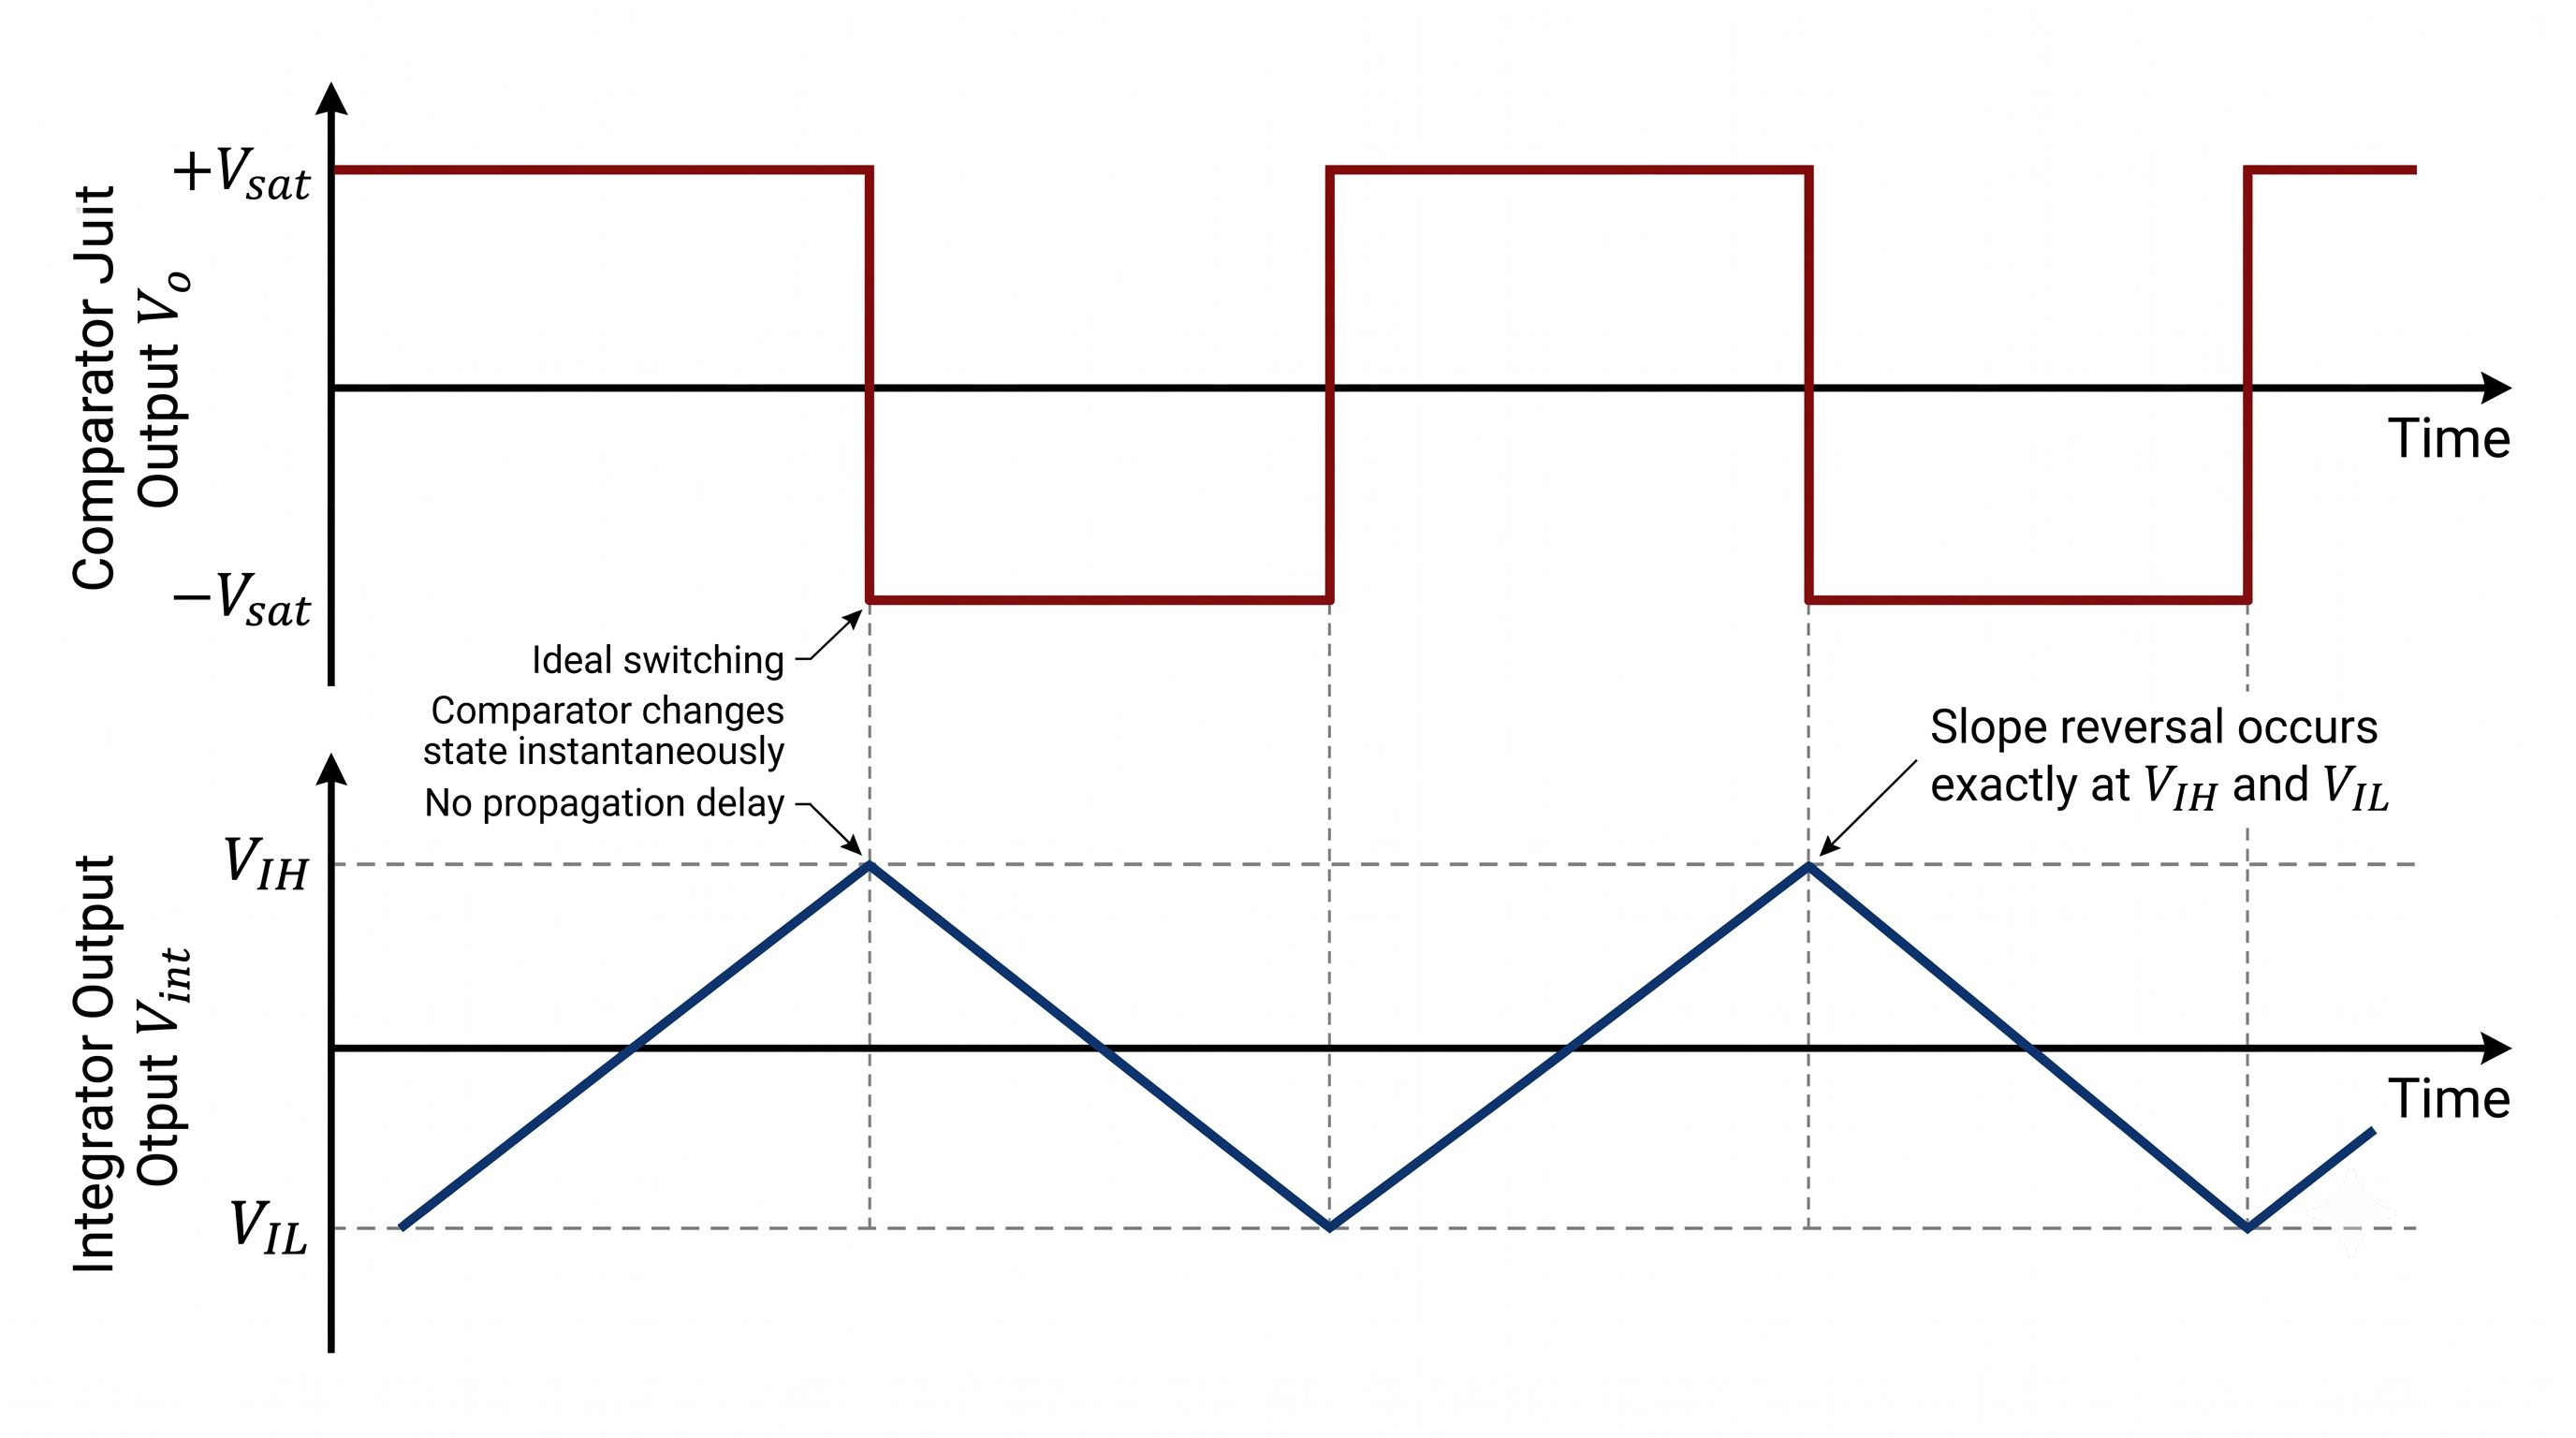
\includegraphics[width = 0.7\textwidth]{img/modif-pwm/comparador-ideal.png}
    \caption{Como se vería al commutar instanáneamente.}
    \label{fig:comparador-ideal}
\end{figure}

Para el circuito, la frecuencia ideal queda dada por
\begin{equation*}
    f_0 = \frac{1}{4RC}\frac{R_{f1}}{R_{f2}}\,.
\end{equation*}
O, equivalentemente, el período ideal es
\begin{equation*}
    T_0 = 4RC\frac{R_{f2}}{R_{f1}}\,,
\end{equation*}
donde, si se reemplaza con los valores obetenidos de resistencias y capacitor ($R_{f1}=\SI{560}{\kilo\ohm}$, $R_{f2}=\SI{56}{\kilo\ohm}$, $R=\SI{220}{\kilo\ohm}$ y $C=\SI{56}{\pico\farad}$) queda de la siquiente manera:
\begin{equation*}
    T_0 \approx \SI{4.93}{\micro\second} \, .
\end{equation*}


Por lo tanto,
\begin{equation*}
    f_0 = \frac{1}{T_0} \approx \SI{202.9}{\kilo\hertz} \, .
\end{equation*}

Este resultado corresponde al caso ideal, donde el tiempo de propagación del
comparador se considera nulo.

Sin embargo, en la medición se observa que la frecuencia de oscilación no es
$202,9\,\text{kHz}$, sino aproximadamente $f_{medida} \approx \SI{129.5}{\kilo\hertz}$.


Esto implica un período simulado de $T_{medido} = \frac{1}{f_{medida}} \approx 7,72\,\upmu$s.

La diferencia entre la frecuencia ideal y la observada se debe principalmente al
tiempo de propagación del comparador LM393. A partir de la medición de este tiempo de propagación con el osciloscopio se obtuvo
\begin{equation*}
    t_p \approx \SI{0.6}{\micro\second} \, .
\end{equation*}

Este tiempo se midió a partir de la observación de las entradas del comparador, la entrada roja es la $V_{ref}$, cuando la celeste supera a la tensión de referencia, la salida debería cambiar a $V_{CC}$, pero se observa que tarda un poco en realizar ese cambio (ver Figura~\ref{fig:tiempo-propagacion}).

\begin{figure}[H]
    \centering
    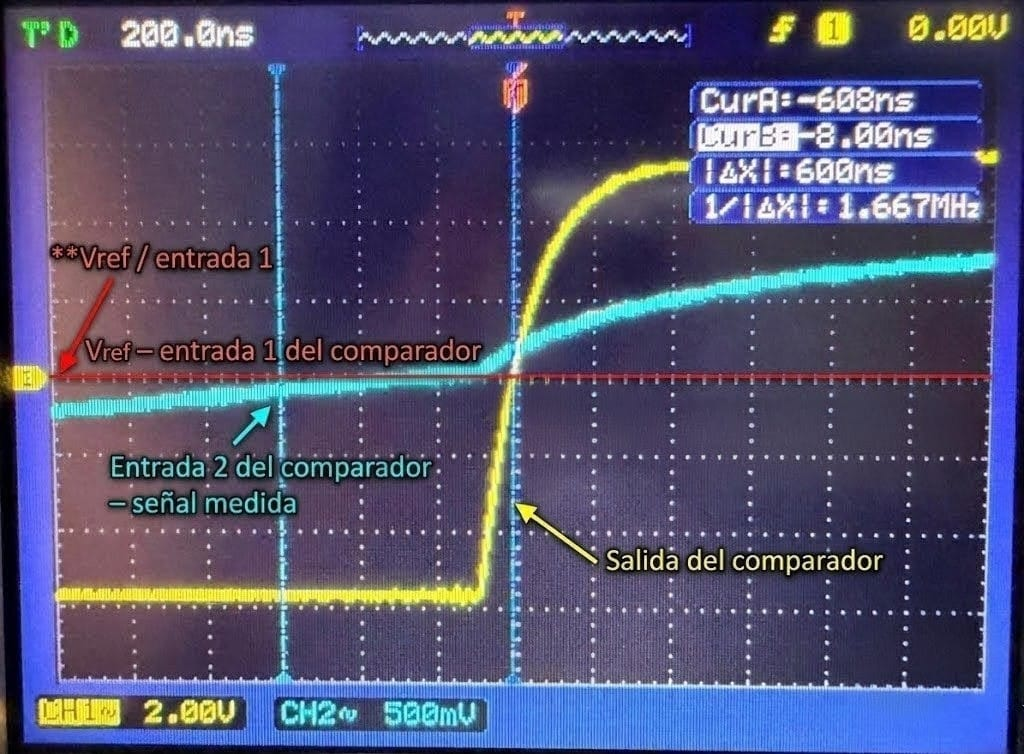
\includegraphics[width = 0.7\textwidth]{img/modif-pwm/tiempo-de-propagacion.jpeg}
    \caption{Tiempo de propagación del comparador LM393 medido con el osciloscopio.}
    \label{fig:tiempo-propagacion}
\end{figure}

La idea importante es que el comparador no cambia su salida exactamente en el
instante en que la señal cruza el umbral de $V_\text{REF}$. La salida del comparador recién conmuta un tiempo $t_p$ después. Durante ese intervalo, el integrador sigue integrando en el mismo sentido.

Por ejemplo, si la triangular está bajando y cruza $V_{IL}$, el comparador
debería cambiar su salida en ese instante. Pero como existe un retardo $t_p$, la
salida todavía no cambia y el integrador sigue haciendo bajar la triangular.
Entonces la señal no se detiene en $V_{IL}$, sino que se pasa por debajo de ese
valor. Lo mismo ocurre cuando la triangular sube y cruza $V_{IH}$: durante el
tiempo de propagación, sigue subiendo y se pasa por encima del umbral.

Ese sobrepaso puede estimarse como: $\Delta V_{over} = m \cdot t_p.$

Donde $m$ es la pendiente de la señal triangular. En este caso, como el
circuito está centrado alrededor de $V_\text{REF}$ y las pendientes de subida y bajada
son aproximadamente iguales, se puede estimar
\begin{equation*}
    m \approx \frac{V_{CC}/2}{RC} \, .
\end{equation*}

Tomando $V_{CC}=\SI{9.1}{\volt}$, se obtiene una pendiente $m \approx 0,369\frac{\text{V}}{\upmu\text{s}}$.

Entonces, para $t_p = \SI{0.6}{\micro\second}$, se obtiene una $\Delta V_{over} \approx \SI{0.22}{\volt}$.

Este valor no es despreciable frente a la histéresis ideal del disparador
Schmitt. La diferencia ideal entre los umbrales es aproximadamente
\begin{equation*}
    V_{IH}-V_{IL} \approx \frac{R_{f2}}{R_{f1}}V_{CC}\,;
\end{equation*}
\begin{equation*}
    V_{IH}-V_{IL} \approx \SI{0.91}{\volt} \, .
\end{equation*}

Pero por el tiempo de propagación, la triangular se pasa aproximadamente
$\SI{0.22}{\volt}$ en cada extremo. Por lo tanto, la excursión efectiva de la triangular
ya no es solamente $\SI{0.91}{\volt}$, sino

\begin{equation*}
    \Delta V_{eff} \approx 0.91\,\text{V} + 2 \cdot 0.22\,\text{V}\,,
\end{equation*}

\begin{equation*}
    \Delta V_{eff} \approx 1.35V\,.
\end{equation*}

Es decir, el tiempo de propagación hace que la triangular tenga que recorrer una
excursión mayor. Como la pendiente del integrador es prácticamente la misma, si
la señal tiene que recorrer más tensión, tarda más tiempo. Por eso aumenta el
período y baja la frecuencia.

Entonces, por cada conmutación, el retardo efectivo agregado al período es
aproximadamente:

\begin{equation*}
    t_p + t_p = 2t_p
\end{equation*}

Como en un período completo hay dos conmutaciones, una en $V_{IL}$ y otra en
$V_{IH}$, la corrección total queda:

\begin{equation*}
    T \approx T_0 + 4t_p
\end{equation*}

Reemplazando: $T \approx \SI{7.33}{\micro\second}$. Y, por lo tanto, la frecuencia queda: $f \approx 136.5kHz$.

Este valor se acerca mucho más al resultado de la medición, $f_{medida} \approx 129.5kHz$.

La diferencia restante puede explicarse porque el modelo real del comparador no
se comporta como un retardo ideal puro. Además del tiempo de propagación, pueden influir también efectos no ideales, como los tiempos de subida y bajada, posibles diferencias entre el retardo de flanco ascendente y descendente, entre otros.

Por lo tanto, la diferencia entre la frecuencia teórica ideal y la frecuencia
simulada se debe a que el tiempo de propagación del comparador no es despreciable
frente al período de oscilación. En nuestro caso:

\begin{equation*}
    \frac{t_p}{T_0} \approx \frac{\SI{0.6}{\micro\second}}{\SI{4.93}{\micro\second}} \approx 0.12
\end{equation*}

Es decir, el tiempo de propagación representa aproximadamente un $12\%$ del
período ideal. Y, como su efecto aparece aproximadamente cuatro veces por
período, el error total sobre el período es mucho mayor a este.

Para que el tiempo de propagación pudiera despreciarse y producir un error menor
al $10\%$ en el período, debería cumplirse aproximadamente:

\begin{equation*}
    4t_p < 0.1T_0
\end{equation*}

\begin{equation*}
    t_p < 0.025T_0
\end{equation*}

Como $T_0 \approx 4.93\mu s$:

\begin{equation}
    t_p < 0.123\mu s
\end{equation}

Mientras que el tiempo de propagación observado es de aproximadamente
$\SI{0.6}{\micro\second}$, bastante mayor que ese valor. Por lo tanto, no puede despreciarse.

% Indicar la medición del tiempo de propagación del comparador y su debida corrección en LTspice. Indicar nuevos valores de resistencia y/o capacitor para obtener una frecuencia de 120-140 kHz. Indicar modificaciones en el circuito (se cambia el potenciómetro por Vc). No hace falta una nueva etapa que garantice 4 V < Vc < 5 V porque como el comparador integra el error, en algun momento llegara a los valores de la triangular.
\subsection{Diodos de rueda libre}
% Incluir análisis de los diodos en el switching.
Las llaves M1 y M2 de la \textit{buck} se implementan con dos MOSFET de forma tal que el circuito conmute. Cuando M1 está cerrada y M2 está abierta, la corriente circula por la malla general y el inductor tiene una polaridad positiva en el nodo de conmutación. Pero, cuando M1 se abre, M2 permanece momentáneamente abierta, abriendo el circuito por completo. Para ello, se coloca un diodo de rueda libre en paralelo al MOS que le otorga un camino alternativo a la corriente para que circule por la malla y permitiendo que el inductor invierta su polaridad (conmuta).

En estos casos, en el momento de la conmutación se producen corrientes que circulan hacia la fuente mediante el MOS M1 que pudieran dañar el diodo intrínseco del mismo, por lo que se le conecta en paralelo otro diodo de rueda libre para evitarlo.

Se escogen diodos Schottky para esta función debido a su baja caída de tensión directa, lo que reduce las pérdidas de conducción durante los intervalos en los que circula la corriente de rueda libre. Además, presentan una recuperación inversa prácticamente nula, característica importante en una fuente conmutada, ya que disminuye los picos de corriente y las pérdidas asociadas al cambio de estado. De esta manera, se mejora la eficiencia del convertidor y se reducen las exigencias eléctricas sobre los MOSFET durante la conmutación.
\subsection{Carga fantasma}
% Mencionar para qué sirve y el agregado del led.
Con el fin de garantizar una corriente mínima de salida durante los ensayos experimentales, se incorporó una carga fantasma compuesta por un diodo LED y su correspondiente resistencia limitadora de corriente. En los convertidores \textit{buck}, especialmente cuando operan en lazo cerrado, una carga mínima contribuye a mantener una regulación estable de la tensión de salida y evita comportamientos indeseados asociados al funcionamiento en vacío, como oscilaciones o una regulación deficiente. Además, el LED proporciona una indicación visual inmediata del correcto funcionamiento de la fuente, permitiendo verificar de manera sencilla la presencia de tensión en la salida durante las pruebas.
\subsection{Capacitores}
% Incluir gráfico de la capacidad vs. la frecuencia. Mencionar que se escoge un capacitor más grande. Incluir capacitor cerámico en paralelo para disminuir la ESR.
Para el capacitor de salida se utilizó un capacitor electrolítico de 
\(10\,\mu\text{F}\). En la hoja de datos se observa que la capacitancia real 
no se mantiene constante con la frecuencia, sino que está especificada respecto 
de \(C_0\), medida a \(20^\circ\text{C}\) y \(100\,\text{Hz}\) (ver \cite{Vishay_030031AS}.). Como se ve en la 
Figura~\ref{fig:cap_vs_freq}, a frecuencias altas la capacitancia efectiva disminuye 
de forma apreciable.

\begin{figure}[H]
    \centering
    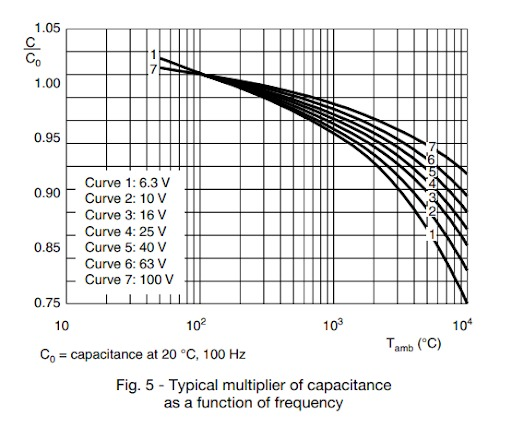
\includegraphics[width=0.65\textwidth]{img/PCB/capacitancia-vs-frecuencia.jpeg}
    \caption{Variación típica de la capacitancia efectiva normalizada respecto 
    de \(C_0\) en función de la frecuencia.}
    \label{fig:cap_vs_freq}
\end{figure}

Esto es importante porque la \textit{buck} opera con una frecuencia de conmutación del 
orden de $f_s \simeq 130\,\text{kHz}$.


Por lo tanto, el capacitor real no se comporta igual que el capacitor ideal de 
\(10\,\mu\text{F}\) usado en la simulación. En el modelo ideal, la corriente 
triangular del inductor es integrada por el capacitor.

\[
i_C(t)=C\frac{dv_o(t)}{dt}
\]

Por lo que el \textit{ripple} de tensión resulta más suavizado. En el circuito real se 
agregó además un capacitor cerámico de \(100\,\text{nF}\) en paralelo, con el 
objetivo de reducir la impedancia equivalente a altas frecuencias. Este capacitor 
ayuda a filtrar componentes rápidas y picos de conmutación, pero no reemplaza la 
función del capacitor electrolítico como elemento principal de almacenamiento de 
energía.

De esta forma, la diferencia entre la simulación y la medición puede explicarse 
porque el capacitor de salida no presenta una capacitancia efectiva constante a la 
frecuencia de trabajo. Como consecuencia, el ripple de salida puede verse menos 
integrado que en el modelo ideal, tomando una forma más triangular o tipo diente 
de sierra.
\subsection{\textit{Gate driver}}
% Explicar para que funciona e incluir los cálculos del diodo y capacitor de boostrap.

En el dieño de convertidores \textit{buck} es necesario añadir una etapa intermedia entre la señal PWM y los \textit{gates} de los transistores MOSFET por varias razones. La primera de ellas es que la salida de dicha etapa no es capaz de alcanzar los niveles de tensión necesarios para poner a los transistores en modo saturación. Además, es necesario cargar y descargar los capaciotres de los MOSFET para que estos puedan abrirse o cerrarse, por lo que se requien picos de corriente para alimentarlos. Por último, es necesario asegurar que ambos MOSFET nunca estén abiertos a la vez, por lo que se necesita implementar un tiempo muerto entre la conmutación de ambas llaves. Estas tres funciones serán cumplidas por la etapa del \textit{gate driver}, la cual se implementa con el circuito integrado IR2104.

\begin{figure}[H]
    \centering
    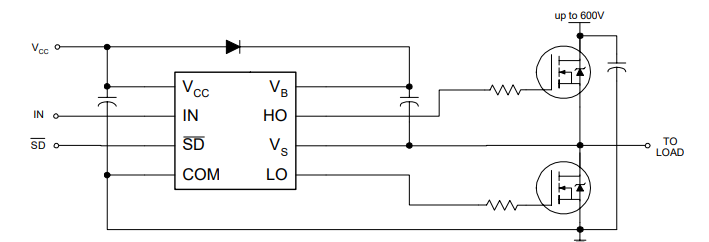
\includegraphics[width=0.8\textwidth]{img/gate driver/circuito GD.png}
    \caption{Circuito del \textit{gate driver}.}
    \label{fig:circuito GD}
\end{figure}

La \autoref{fig:circuito GD} fue extraída de la hoja de datos del integrado y muestra el circuito a implementar. El capacitor entre las entradas $V_B$ y $V_S$ es el capacitor de \textit{bootstrap}, el cual almacena la carga con la que se alimentará a los capacitores del MOSFET superior para que empiece a conducir. El diodo de \textit{bootstrap} permite que el capacitor se cargue a través de $V_{CC}$ en un semiciclo y fuerza a que su carga vaya al \textit{gate} en el otro. Por lo tanto, dicho diodo debe ser capaz de operar correctamente a la frecuencia de conmutación del circuito, por lo que se decidió utilizar los diodos Schottky antes mencionados (1N5822). 

El capacitor de \textit{bootstrap} no puede tener un valor arbitrario, debe tener un mínimo valor suficiente para cargar la compurta del transistor superior. Se impone entonces la siguiente restriccióna su capacidad:
\begin{equation*}
    C_{boot} > 10 \cdot \frac{Q}{V_{CC} - V_d} \,,
\end{equation*}
donde $Q$ es la carga de la compuerta del transistor y $V_d$ es la tensión de caída del diodo. Esta restricción asegura que el capacitor nunca se descargue completamente. De la hoja de datos del transistor se obtiene $Q = \SI{62}{\nano \coulomb}$, y con $V_{CC} = \SI{10}{\volt}$ y $V_d = \SI{0,2}{\volt}$ se tiene que $C_{boot} > \SI{63.2}{\nano \farad}$. De esta forma, se eligió $C_{boot} = \SI{100}{\nano \farad}$ para tener ciero margen.

A la hora de añadir el \textit{gate driver} a la placa fue necesario hacer modificaciones a la misma. Tanto el generador de  PWM como la etapa de compensación son alimentados por un regulador LM7809, el cual entrega $\SI{9}{\volt}$. Sin embargo, la hoja de datos del IR2104 informa que el mismo debe ser alimentado con $\SI{10}{\volt}$ o más, lo que fue comprobado experimentalmente.

\begin{minipage}{0.45\textwidth}
    \begin{figure}[H]
        \centering
        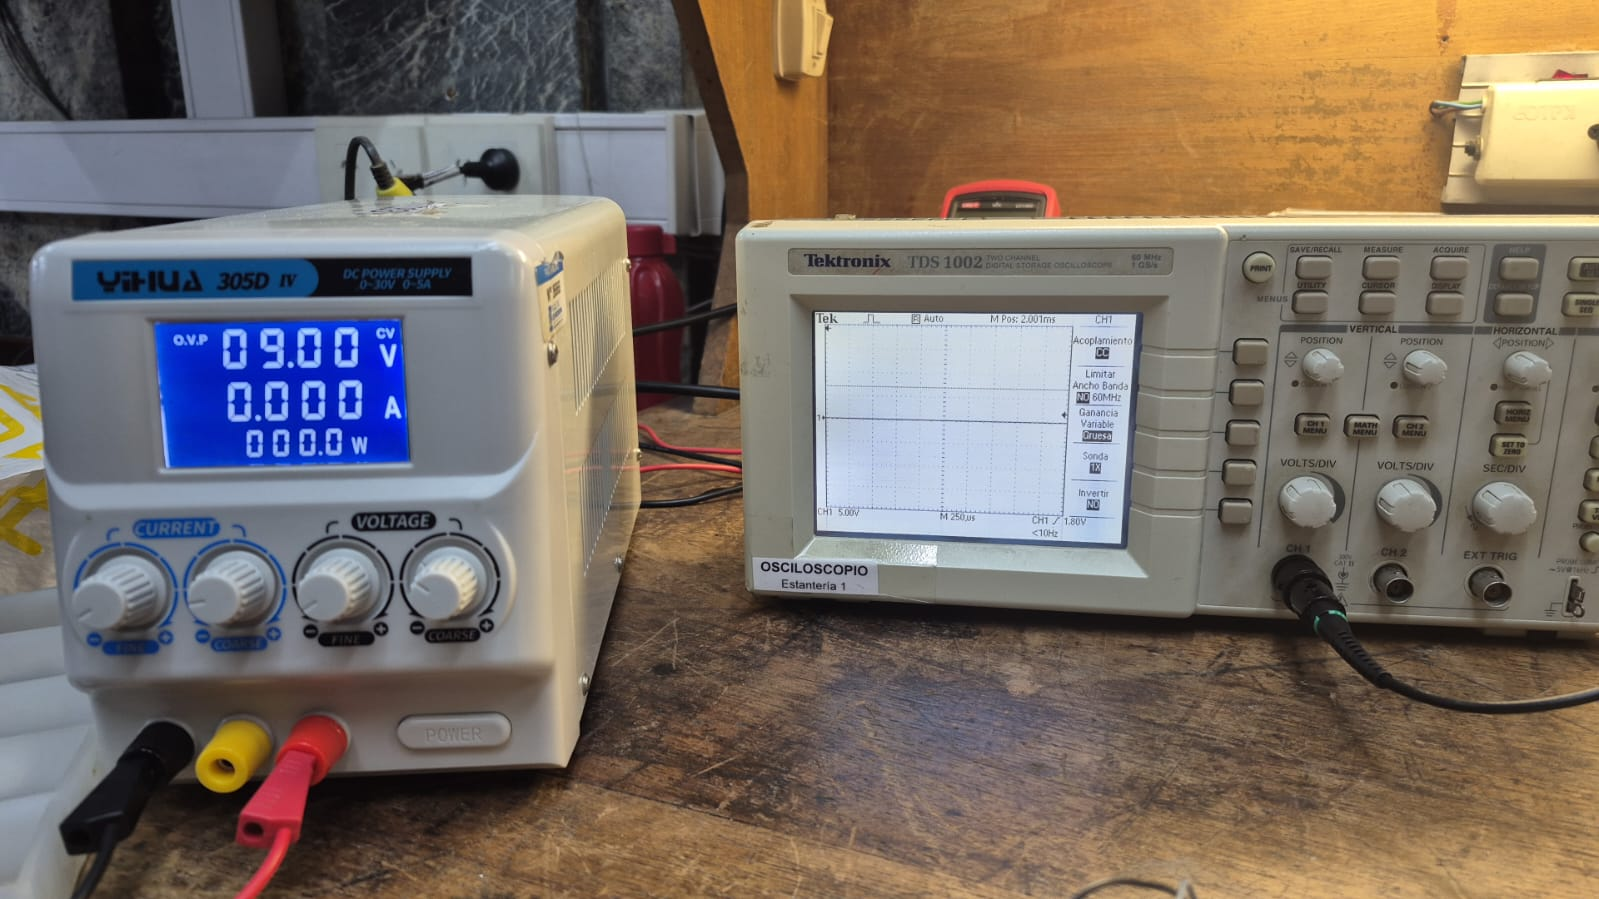
\includegraphics[width=0.9\textwidth]{img/gate driver/GD_9V.png}
        \caption{\textit{Gate driver} alimentado con $9\,$V.}
        \label{fig:GD 9V}
    \end{figure}
\end{minipage}
\begin{minipage}{0.45\textwidth}
    \begin{figure}[H]
        \centering
        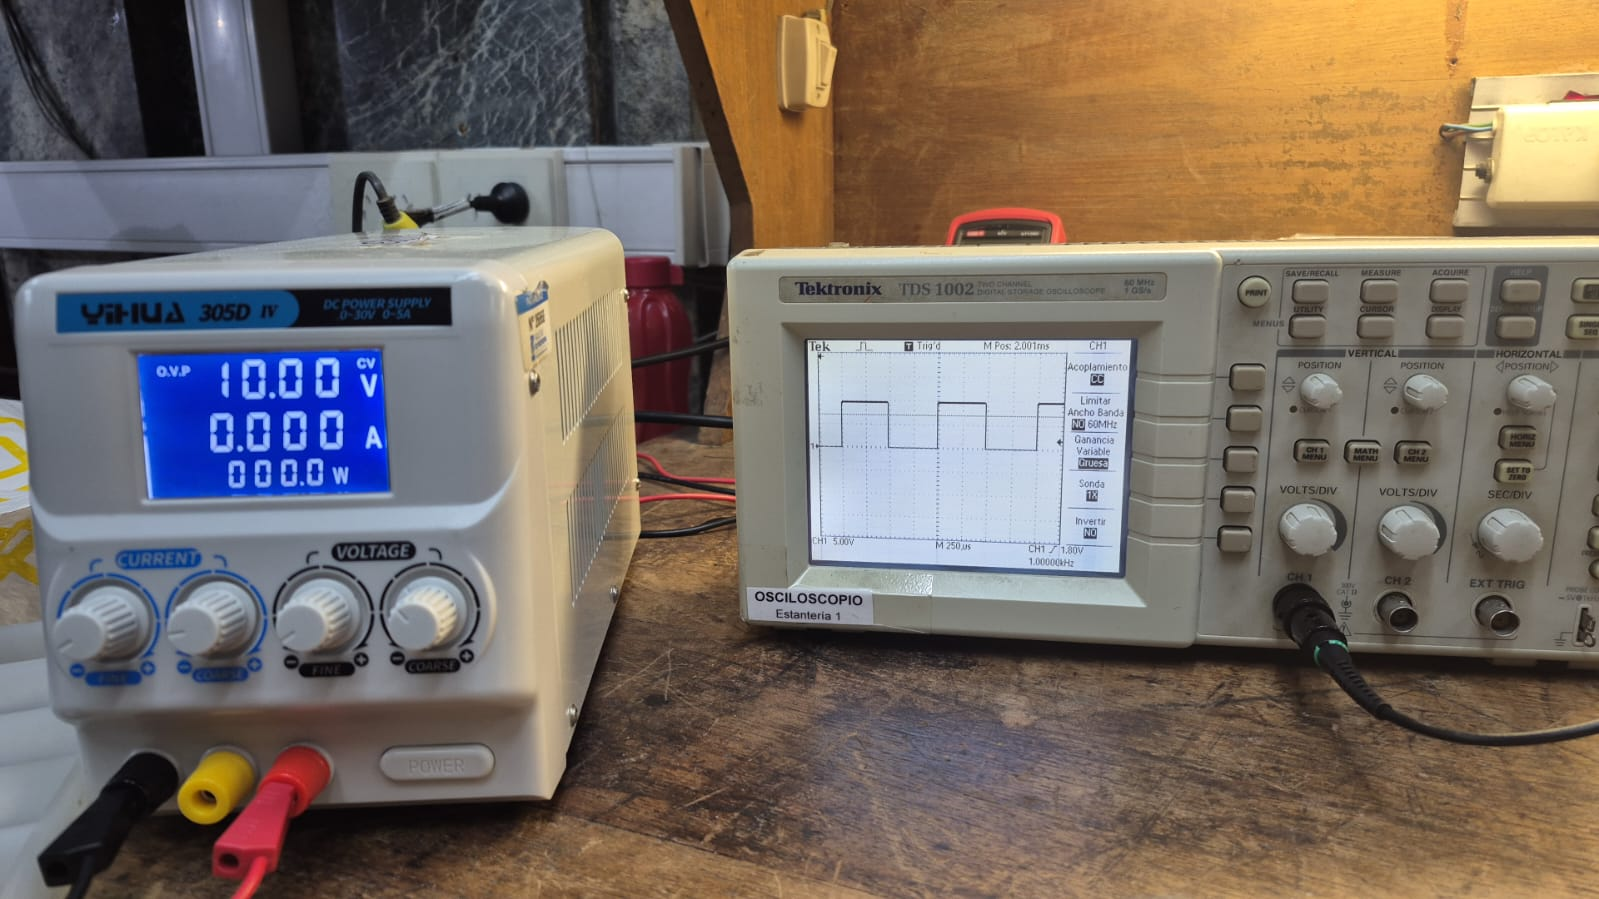
\includegraphics[width=0.9\textwidth]{img/gate driver/GD_10V.png}
        \caption{\textit{Gate driver} alimentado con $10\,$V.}
        \label{fig:GD 10V}
    \end{figure}
\end{minipage}

Se alimentó el \textit{gate driver} con $\SI{9}{\volt}$ y $\SI{10}{\volt}$ y se midió una de sus salidas con un osciloscopio. En las Figuras \ref{fig:GD 9V} y \ref{fig:GD 10V} se ecuentra el resultado del experimento, y puede comprobarse que en la pantalla del osciloscopio se obtiene una señal cuadrada a la salida solo si se alimenta al integrado con $\SI{10}{\volt}$ o más.


\subsection{Red de compensación}
% Hablar de la red de compensación tipo III y cómo se calcularon sus componentes (Agregar en un apéndice los cálculos matriciales).
Según la nota de aplicación de Linear Technology~\cite{Zhang2015}, la transferencia de $\hat{d}$ a $\hat{v}_o$ para un convertidor \textit{buck} es
\[
    G_{dv}(s) = \frac{\hat{v}_o}{\hat{d}} = V_{IN} \cdot \frac{1 + s/\omega_{z\text{-ESR}}}{1 + \dfrac{s}{Q\omega_0} + \dfrac{s^2}{\omega_0^2}} \, ,
\]
donde los parámetros de la planta son
\begin{align*}
    \omega_{z\text{-ESR}} &= \frac{1}{r_C \cdot C} \, , \\[6pt]
    \omega_0 &= 2\pi f_0 = \frac{1}{\sqrt{L \cdot C}} \cdot \sqrt{\frac{1 + r_L/R}{1 + r_C/R}} \;\approx\; \frac{1}{\sqrt{L \cdot C}} \, , \\[6pt]
    Q &= \frac{1}{\omega_0} \cdot \frac{1}{\dfrac{L}{r_L + R} + C\left(r_C + r_L \!\parallel\! R\right)} \;\approx\; \sqrt{L \cdot C} \cdot \frac{1}{\dfrac{L}{R} + C(r_C + r_L)} \, .
\end{align*}
La linealización es válida si $r_L \ll R$ y $r_C \ll R$, condición que se cumple en el diseño dado que la carga mínima es de $6\,\Omega$ ($9{.}3\,\text{V}/1{.}6\,\text{A} \approx 5{.}8\,\Omega$). En resumen, el sistema tiene un cero real ($\omega_{z\text{-ESR}}$) y un par de polos complejos conjugados de resonancia ($\omega_0$, $Q$). Notar que esto es una linealización alrededor de un punto de equilibrio usando un modelo promediado.

\begin{figure}[H]
    \centering
    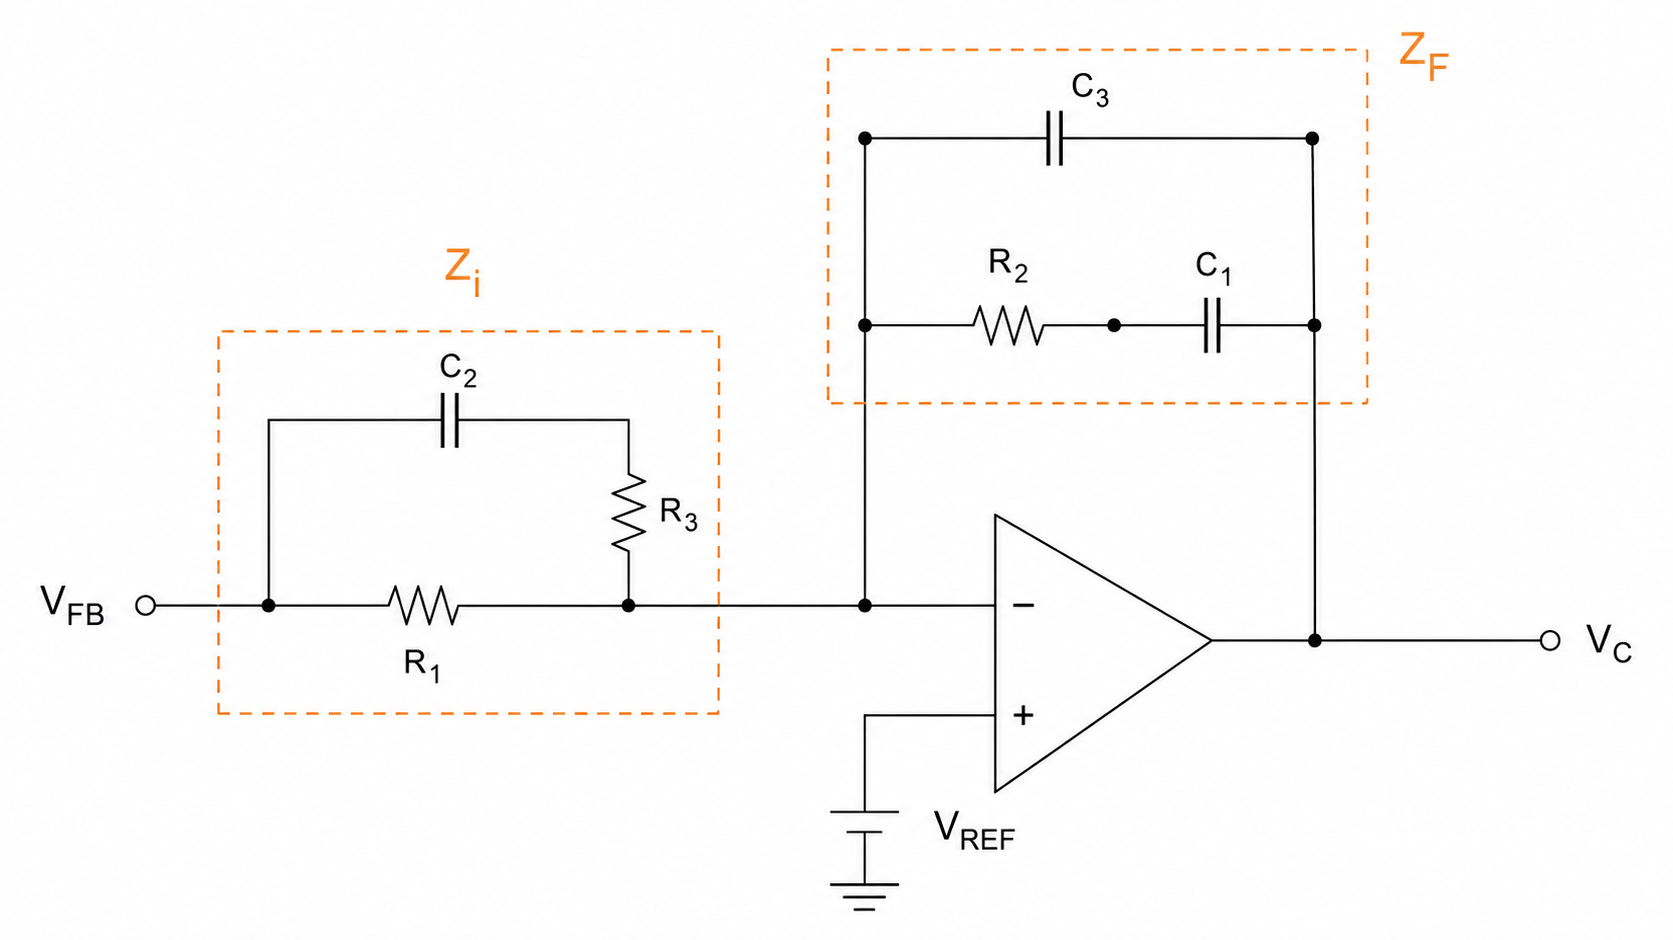
\includegraphics[width = 0.8\textwidth]{img/red_compensacion.png}
    \caption{Red de compensación tipo III.}
    \label{fig:red_compensacion}
\end{figure}

Se propone una red de compensación tipo III (véase la Figura~\ref{fig:red_compensacion}). Llamando $Z_i$ y $Z_f$ a la impedancia de entrada y de retroalimentación respectivamente se tiene
\[
    A(s) = \frac{V_c(s)}{V_{FB}(s)} = -\frac{Z_f}{Z_i}
\]
con
\[
    Z_i = R_1 \,\Big\|\, \left(R_3 + \frac{1}{C_2 s}\right) \quad \text{y} \quad
    Z_f = \frac{1}{C_3 s} \,\Big\|\, \left(R_2 + \frac{1}{C_1 s}\right) \, .
\]

Recordando que $R + \dfrac{1}{Cs} = \dfrac{RCs + 1}{Cs} = R \cdot \dfrac{s + 1/RC}{s}$, la función de transferencia del compensador resulta ser un integrador con 2 polos y 2 ceros:
\[
    A(s) = -\frac{\omega_1}{s} \cdot \frac{\left(1 + s/\omega_{z_1}\right)\left(1 + s/\omega_{z_2}\right)}{\left(1 + s/\omega_{p_1}\right)\left(1 + s/\omega_{p_2}\right)} \, ,
\]
donde los ceros, polos y ganancia del integrador quedan determinados por los componentes según
\begin{align}
    \omega_1    &= \frac{1}{R_1(C_1 + C_3)}\,;  \label{eq:w1} \\[4pt]
    \omega_{z_1} &= \frac{1}{R_2 C_1}          \quad \text{(cero de $Z_f$, cuando $Z_f \to 0$)}\,; \label{eq:wz1} \\[4pt]
    \omega_{z_2} &= \frac{1}{(R_1 + R_3)C_2}   \quad \text{(cero de $Z_i$, cuando $Z_i \to \infty$)}\,; \label{eq:wz2} \\[4pt]
    \omega_{p_1} &= \frac{1}{R_3 C_2}           \quad \text{(polo de $Z_i$, cuando $Z_i \to 0$)}\,; \label{eq:wp1} \\[4pt]
    \omega_{p_2} &= \frac{1}{R_2 \,\dfrac{C_1 C_3}{C_1 + C_3}} \quad \text{(polo de $Z_f$, cuando $Z_f \to 0$)}\,; \label{eq:wp2}
\end{align}
siendo $\omega_1$ la frecuencia a la cual la ganancia del integrador llega a $0\,\text{dB}$ (frecuencia de cruce o ancho de banda).

La observación clave es que por la construcción del modulador PWM, $V_c$ debe encontrarse entre $4\,\text{V}$ y $5\,\text{V}$. La relación entre el \textit{duty cycle} y la tensión de control es lineal:
\[
    d = \frac{V_c - 4\,\text{V}}{5\,\text{V} - 4\,\text{V}} \, ,
\]
por lo que $\hat{d} \approx \hat{v}_c$ y la transferencia del compensador referida a $\hat{v}_o$ es
\[
    \frac{\hat{v}_c}{\hat{v}_o}(s) = -\frac{\omega_1}{s} \cdot \frac{\left(1 + s/\omega_{z_1}\right)\left(1 + s/\omega_{z_2}\right)}{\left(1 + s/\omega_{p_1}\right)\left(1 + s/\omega_{p_2}\right)} \,.
\]

Las restricciones de diseño que impone la estrategia de cancelación son las siguientes.

\begin{enumerate}
    \item \textbf{Cancelación del polo doble de resonancia} ($\omega_{z_1} = \omega_{z_2} = \omega_0$).
    \[
        \frac{1}{R_2 C_1} = \frac{1}{(R_1 + R_3)C_2} = \frac{1}{\sqrt{LC}}
    \]

    \item \textbf{Cancelación del cero de la ESR} ($\omega_{p_1} = \omega_{z\text{-ESR}}$).
    \[
        \frac{1}{R_3 C_2} = \frac{1}{r_C \cdot C}
    \]

    \item \textbf{Filtrado del ruido de conmutación} ($\omega_{p_2} = 2\pi f_{sw}/k$, con $k = 10$).
    \[
        \frac{1}{R_2 \,\dfrac{C_1 C_3}{C_1 + C_3}} = \frac{2\pi f_{sw}}{10} \approx 82\,000\,\text{rad/s}
    \]
\end{enumerate}

Se tienen 5 restricciones y 6 incógnitas ($R_1, R_2, R_3, C_1, C_2, C_3$), por lo que el sistema tiene \textbf{1 grado de libertad}. Aplicando logaritmo a cada una de las relaciones~\eqref{eq:w1}--\eqref{eq:wp2}, el sistema se vuelve lineal en las variables $x_i = \ln(\cdot)$. Definiendo
\[
    \mathbf{x} = \begin{bmatrix} \ln R_1 \\ \ln R_2 \\ \ln R_3 \\ \ln C_1 \\ \ln C_2 \\ \ln C_3 \end{bmatrix} \quad \text{e} \quad
    \mathbf{y} = \begin{bmatrix} \ln \omega_1 \\ \ln \omega_{z_1} \\ \ln \omega_{z_2} \\ \ln \omega_{p_1} \\ \ln \omega_{p_2} \end{bmatrix}
\]
el sistema $\mathbf{y} = A\,\mathbf{x}$ tiene la siguiente forma (bajo la aproximación $R_1 \gg R_3$, $C_1 \gg C_3$).

\begin{equation*}
    \begin{pmatrix} \ln \omega_1 \\ \ln \omega_{z_1} \\ \ln \omega_{z_2} \\ \ln \omega_{p_1} \\ \ln \omega_{p_2} \end{pmatrix}
    =
    \begin{pmatrix}
        -1 & 0  & 0  & -1 & 0  & 0  \\
         0 & -1 & 0  & -1 & 0  & 0  \\
        -1 & 0  & 0  & 0  & -1 & 0  \\
         0 & 0  & -1 & 0  & -1 & 0  \\
         0 & -1 & 0  & 0  & 0  & -1
    \end{pmatrix}
    \begin{pmatrix} \ln R_1 \\ \ln R_2 \\ \ln R_3 \\ \ln C_1 \\ \ln C_2 \\ \ln C_3 \end{pmatrix}
\end{equation*}

Se puede verificar que el núcleo de $A$ está generado por
\[
    \mathbf{N}_0 = \begin{pmatrix} 1 \\ 1 \\ 1 \\ -1 \\ -1 \\ -1 \end{pmatrix}
    \qquad \text{ya que} \qquad A\,\mathbf{N}_0 = \mathbf{0} \,.\quad \checkmark
\]

Por lo tanto, el conjunto de soluciones forma una recta: si $\mathbf{x}_0$ es solución, entonces $\mathbf{x}_0 + \alpha\,\mathbf{N}_0$ también lo es para todo $\alpha \in \mathbb{R}$.

Para evitar trabajar con valores numéricos muy extremos, se expresan las resistencias en k$\Omega$ y los capacitores en nF. En ese caso, $RC = R[\text{k}\Omega] \cdot 10^3 \cdot C[\text{nF}] \cdot 10^{-9} = \frac{R[\text{k}\Omega]\,C[\text{nF}]}{10^6}$, con lo que
\[
    \omega = \frac{10^6}{R[\text{k}\Omega]\,C[\text{nF}]}
\]
y el sistema lineal logarítmico resulta
\begin{align*}
    \ln \omega_1    - \ln(10^6) &= -\ln R_1 - \ln C_1\,; \\
    \ln \omega_{z_1} - \ln(10^6) &= -\ln R_2 - \ln C_1\,; \\
    \ln \omega_{z_2} - \ln(10^6) &= -\ln R_1 - \ln C_2\,; \\
    \ln \omega_{p_1} - \ln(10^6) &= -\ln R_3 - \ln C_2\,; \\
    \ln \omega_{p_2} - \ln(10^6) &= -\ln R_2 - \ln C_3\,.
\end{align*}
Solo cambia el vector $\mathbf{y}$ (se le resta $\ln(10^6)$ a cada componente); la matriz $A$ permanece idéntica.

Sea $\mathbf{x}_0 = \operatorname*{arg\,min}_{\mathbf{x}} \|\mathbf{y} - A\mathbf{x}\|^2$ la solución de mínimos cuadrados al sistema simplificado ($R_1 \gg R_3$, $C_1 \gg C_3$). La familia de soluciones es
\begin{equation*}
    \mathbf{x}_0 + \alpha\,\mathbf{N}_0 = \ln \begin{pmatrix} R_1 \\ R_2 \\ R_3 \\ C_1 \\ C_2 \\ C_3 \end{pmatrix} + \alpha \begin{pmatrix} 1 \\ 1 \\ 1 \\ -1 \\ -1 \\ -1 \end{pmatrix}
    \quad \Rightarrow \quad \ln R_1 + \alpha = \ln(\alpha' R_1) \quad \text{con } \alpha' = e^\alpha \, .
\end{equation*}
Es decir, barrer $\alpha$ equivale a escalar todas las resistencias por $\alpha'$ y todos los capacitores por $1/\alpha'$, con $0{,}1 < \alpha' < 10$ ($\ln 0{,}1 < \alpha < \ln 10$). Barriendo a lo largo de esta recta del núcleo se puede acercar la solución a los valores comerciales preferidos sin introducir error adicional en las frecuencias objetivo.

No mezclar rad/s con Hz en las entradas del sistema; todas las frecuencias deben estar expresadas en las mismas unidades.

El \textit{script} de Python utilizado se encuentra en el siguiente enlace: \url{https://colab.research.google.com/drive/1cBno2bBx_6Jxcf00gmb1MuaoOuErkoNw?usp=sharing$0}.

Los valores finalmente seleccionados son $R_1 = 68\,\text{k}\Omega$, $R_2 = 3.3\,\text{k}\Omega$, $R_3 = 680\,\Omega$, $C_1 = 22\,$nF, $C_2 = 1.2\,$nF y $C_3 = 5.6 \,$nF.

Asimismo, se añadió una resistencia $R_4 = 24\,\text{k}\Omega$ entre $V_{FB}$ y GND que no influye en la compensación ya que en señal queda entre dos tierras; pero, en estado estacionario, la misma forma un divisor resitivo con la resistencia $R_1$ de forma tal que $V_o = V_\text{REF} \cdot (R_1 + R_4)/R_4$.
\subsection{Circuito final}
% Incluir un esquemático del diseño final del circuito.
En base a todo lo comentado en las secciones anteriores, el circuito final queda como se observa en la Figura~\ref{fig:circuito-final}.

\newpage

\begin{figure}[H]
    \centering
    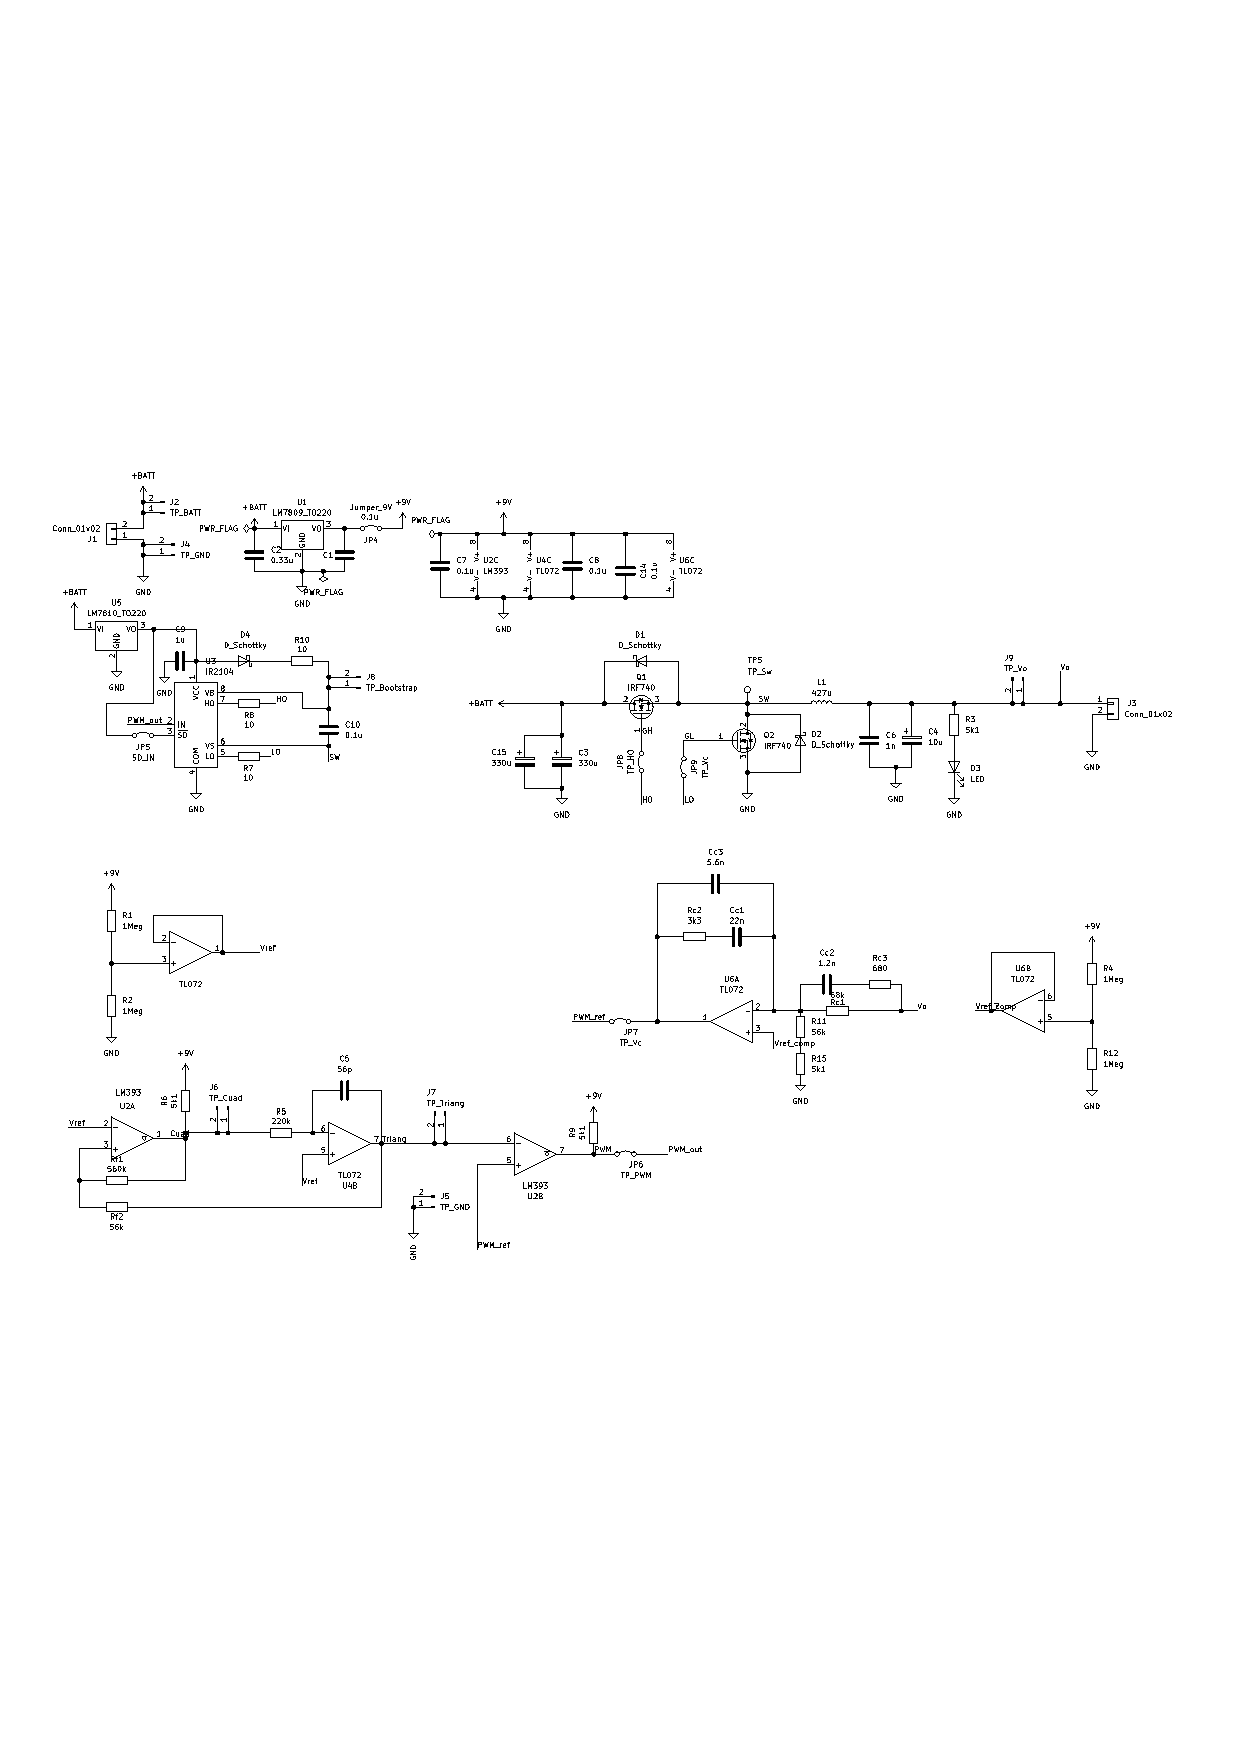
\includegraphics[width = 1\textwidth]{img/PCB/Circuito final.pdf}
    \caption{Circuito final hecho en KiCad.}
    \label{fig:circuito-final}
\end{figure}

\newpage

\section{Simulaciones}
% Incluir gráficos de simulaciones.
En esta sección se detallan las simulaciones hechas para validar el diseño de la red de compensación. En primer lugar, se simuló la respuesta del circuito con realimentación unitaria ante un escalón en la entrada, el cual caía de $\SI{30}{\volt}$ a $\SI{12}{\volt}$. Esta simulación se hizo para verificar si la realimentación unitaria era suficiente para compensar el lazo. La simulación se hizo para los siguientes valores de carga: $R_L = \{6,\ 30, \ 95\}\,\Omega$. Todas las simulaciones fueron hechas con el modelo promediado. 

\begin{figure}[H]
    \centering
    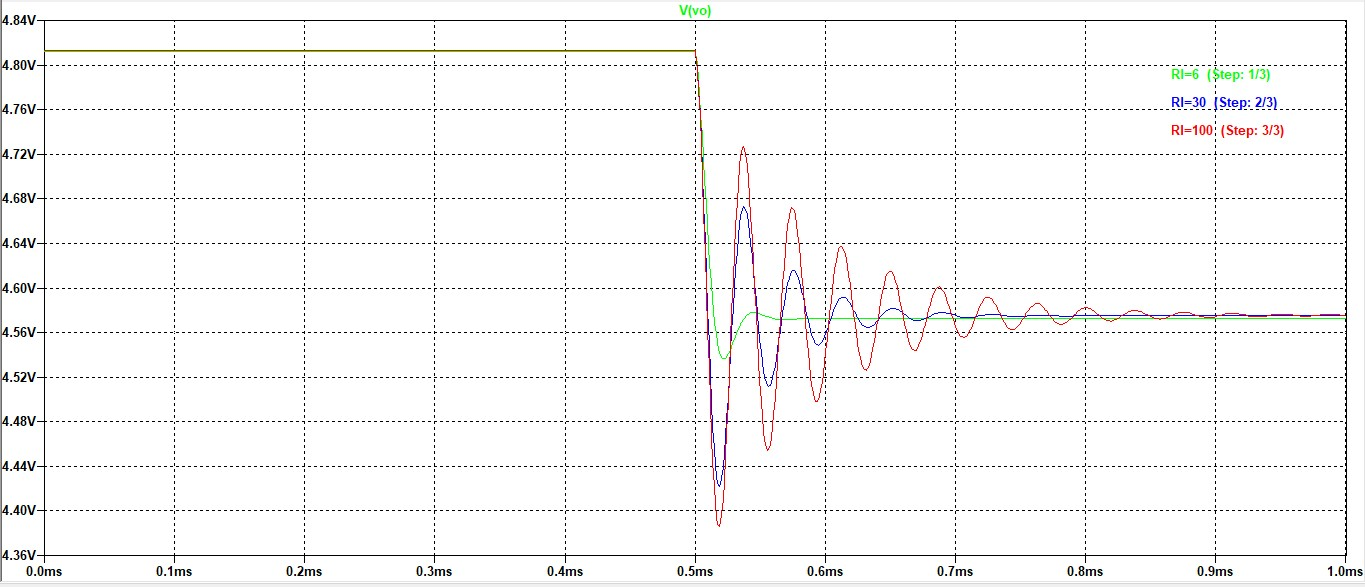
\includegraphics[width=0.9\textwidth]{img/simulacion imagenes/rta temporal-CL-sin compensar.png}
    \caption{Respuesta temporal sin compensar para distintos valores de carga.}
    \label{fig:rta temporal-sin compensar}
\end{figure}

Puede verse en la \autoref{fig:rta temporal-sin compensar} que la respuesta temporal depende fuertemente de la carga, como sugiere la ecuación del factor de calidad $Q$. Dado que la señal es excesivamente oscilante para ciertos valores de carga, es necesario compensar. Además, la salida no se establece en el valor deseado de $\SI{9.5}{\volt}$.

\begin{figure}[H]
    \centering
    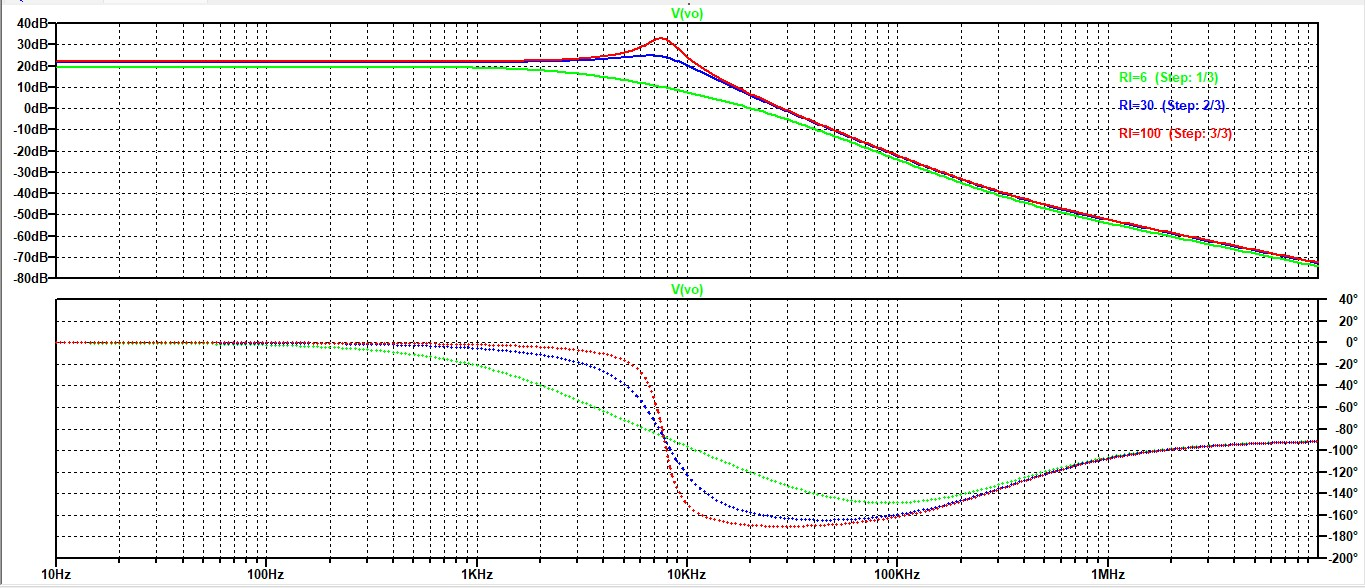
\includegraphics[width=0.9\textwidth]{img/simulacion imagenes/bode-OL.png}
    \caption{Diagrama de Bode a lazo abierto.}
    \label{fig:bode OL}
\end{figure}

La \autoref{fig:bode OL} muestra el diagrama de bode a lazo abierto de la \textit{buck}. Se destaca que a medida que la carga aumenta, el margen de fase decrece, como sugieren los resultados de la \autoref{fig:rta temporal-sin compensar}. Puede notarse el efecto de los polos complejos conjugados alrededor de la frecuencia $f = \SI{7}{\kilo \hertz}$. Estos polos imponen un cambio violento en la fase, lo que hace al sistema más oscilante.

\begin{figure}[H]
    \centering
    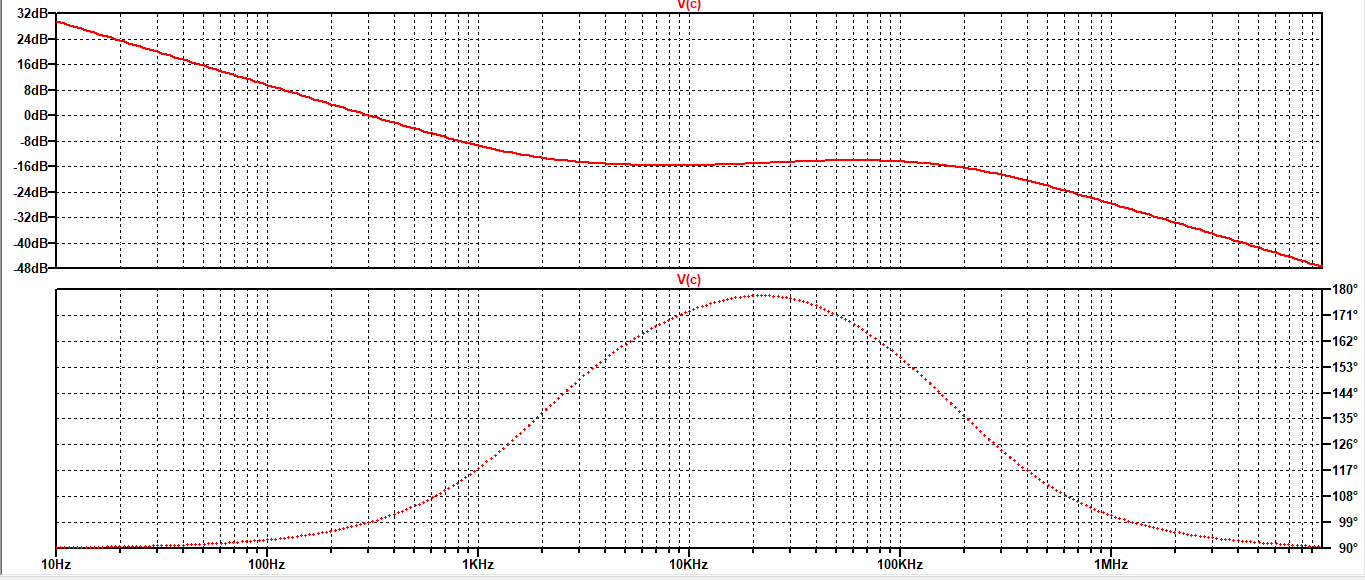
\includegraphics[width=0.9\textwidth]{img/simulacion imagenes/Bode-realimentador.png}
    \caption{Diagrama de Bode de la red de compensación.}
    \label{fig:bode realimentador}
\end{figure}

La \autoref{fig:bode realimentador} muestra el diagrama de Bode de la red de compensación. La misma fue diseñada con los criterios ya mencionados y de forma tal que añadiera fase para la frecuencia $f = \SI{7}{\kilo \hertz}$, mitigando así el efecto de los polos complejos conjugados.

\begin{figure}[H]
    \centering
    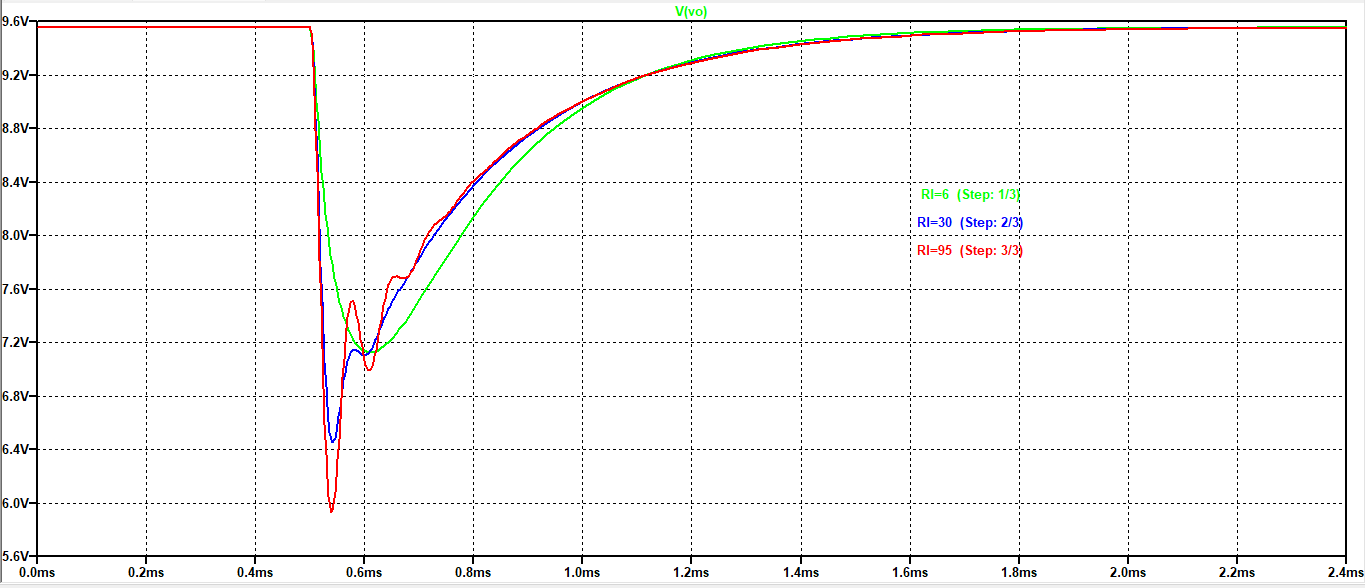
\includegraphics[width=0.9\textwidth]{img/simulacion imagenes/rta temporal-CL-compensado.png}
    \caption{Respuesta temporal del sistema compensado.}
    \label{fig:rta temporal comp}
\end{figure}

La \autoref{fig:rta temporal comp} muestra la respuesta del sistema compensado para el escalón ya mencionado. Se observa que se pudieron reducir las oscilaciones satisfactoriamente y que una vez agregada la compensación el sistema se establece en la tensión deseada. Si bien esta respuesta es un poco lenta, se considera que el tiempo de establecimiento es suficiente para esta aplicación.

\begin{figure}[H]
    \centering
    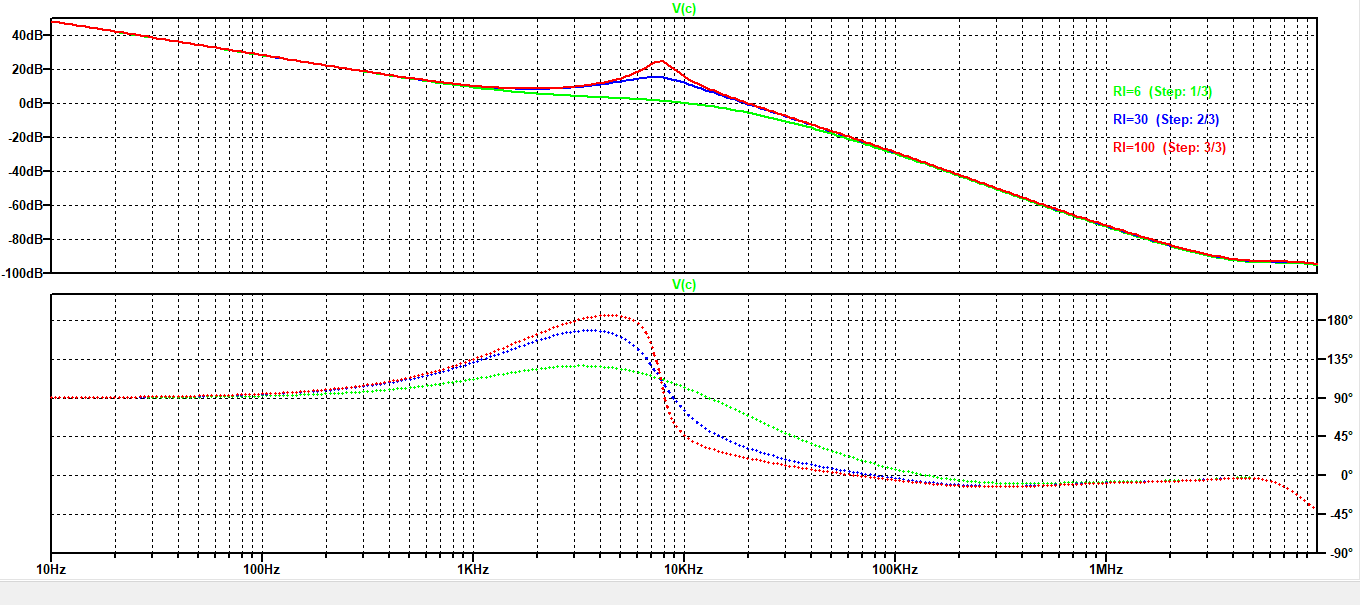
\includegraphics[width=0.9\textwidth]{img/simulacion imagenes/Bode-CL.png}
    \caption{Diagrama de Bode a lazo cerrado.}
    \label{fig:bode CL}
\end{figure}

La \autoref{fig:bode CL} muestra el diagrama de Bode a lazo cerrado para distintos valores de carga. Se observa que incluso en el peor de los casos el sistema presenta un margen de fase elevado (aproxiamdanete $\SI{100}{\degree}$). 

\section{Diseño e implementación del PCB}
\subsection{Diseño}

Una vez compensado el sistema se procedió a diseñar el PCB. Para evitar problemas de interferencia electromagnética se tuvieron en cuenta las recomendaciones detalladas en la hoja de datos del regulador LM2576~\cite{LM2576_datasheet}. 

\begin{figure}[H]
    \centering
    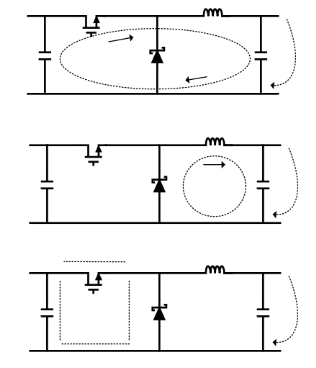
\includegraphics[width=0.9\textwidth]{img/PCB/Mallas.png}
    \caption{Mallas de la fuence \textit{buck}.}
    \label{fig:mallas}
\end{figure}

La mencionada hoja de datos provee la \autoref{fig:mallas} y destaca que la malla de la izquierda (la cual contiene al capacitor de entrada y a ambas llaves) es la más propensa a producir ruido ya que tiene elevados picos de corriente. De esta forma, si las pistas tuvieran una inductancia parásita elevada producirían altos picos de tensión en virtud de la ecuación del inductor 
\[
  v_L = L \frac{di_L}{dt}\,.
\]
Así, incluso con pequeños valores de $L$ se pueden producir picos elevados de $v_L$. Es entonces necesario reducir al máximo la inductancia parásita de las pistas, lo cual se consigue haciéndolas lo más anchas y cortas posibles y minimizando la superficie de la espira que forma la malla de entrada. 

\begin{figure}[H]
    \centering
    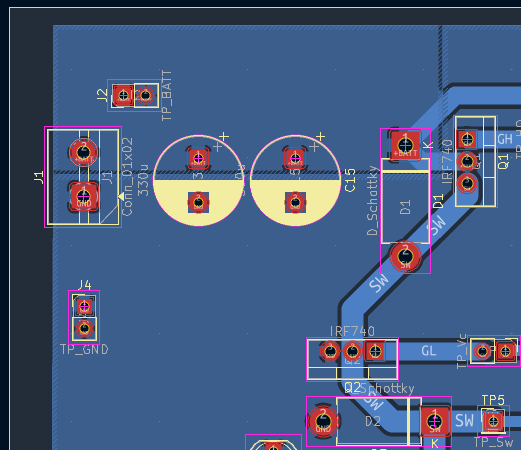
\includegraphics[width=0.9\textwidth]{img/PCB/Malla en el PCB.png}
    \caption{Malla de entrada en el PCB.}
    \label{fig:malla en el PCB}
\end{figure}

La \autoref{fig:malla en el PCB} muestra cómo se implementó la malla de entrada en el PCB, donde los capacitores electrolíticos forman el capacitor de entrada y los transistores $Q_1$ y $Q_2$ forman las llaves. 

\begin{figure}[H]
    \centering
    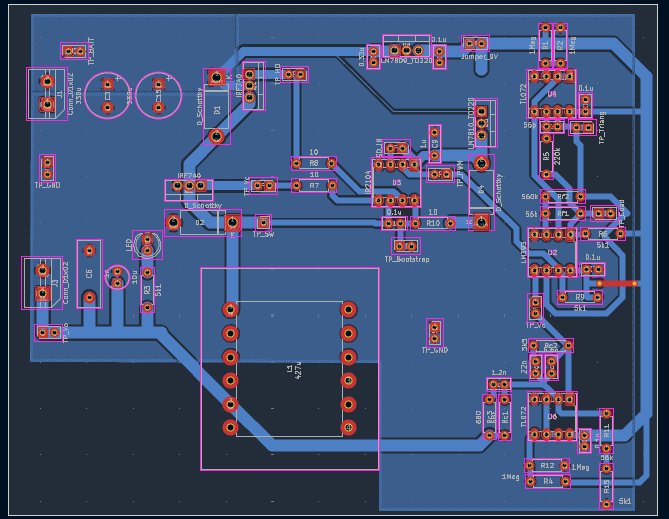
\includegraphics[width=0.9\textwidth]{img/PCB/PCB final.png}
    \caption{PCB final}
    \label{fig:PCB final}
\end{figure}

\begin{figure}[H]
    \centering
    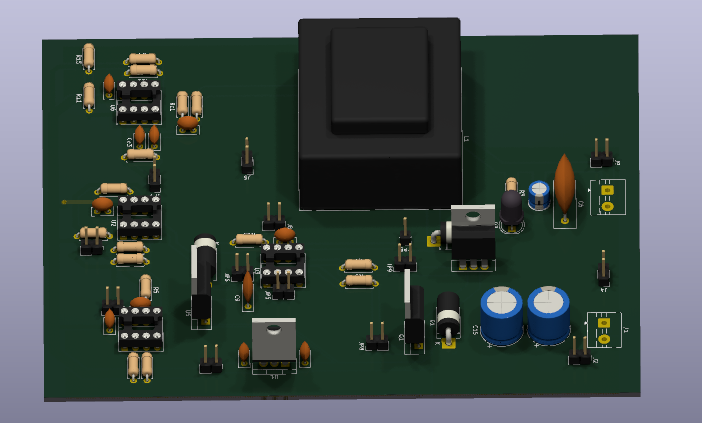
\includegraphics[width=0.9\textwidth]{img/PCB/PCB3D.png}
    \caption{Versión 3D del PCB}
    \label{fig:PCB3D}
\end{figure}

Las Figuras \ref{fig:PCB final} y \ref{fig:PCB3D} muestran el resultado final del diseño del PCB. 

\subsection{Implementación}

Dado que fue imposible delegar la manufactura del PCB por causas de fuerza mayor, la misma formó parte del desarrollo del \textit{checkpoint}.

\begin{figure}[H]
    \centering
    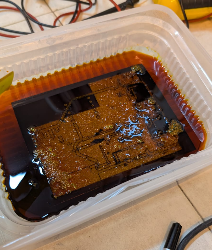
\includegraphics[width=0.9\textwidth]{img/PCB/PCB en acido.png}
    \caption{PCB en ácido.}
    \label{fig:PCB en ácido}
    
\end{figure}

La \autoref{fig:PCB en ácido} muestra el proceso de fabricación. Cabe mencionar que, si bien el mismo llevo más tiempo, también permitió un mayor grado de libertad en cuanto al tamaño de los agujeros y la correción de errores en el diseño original del PCB.

\begin{figure}[H]
    \centering
    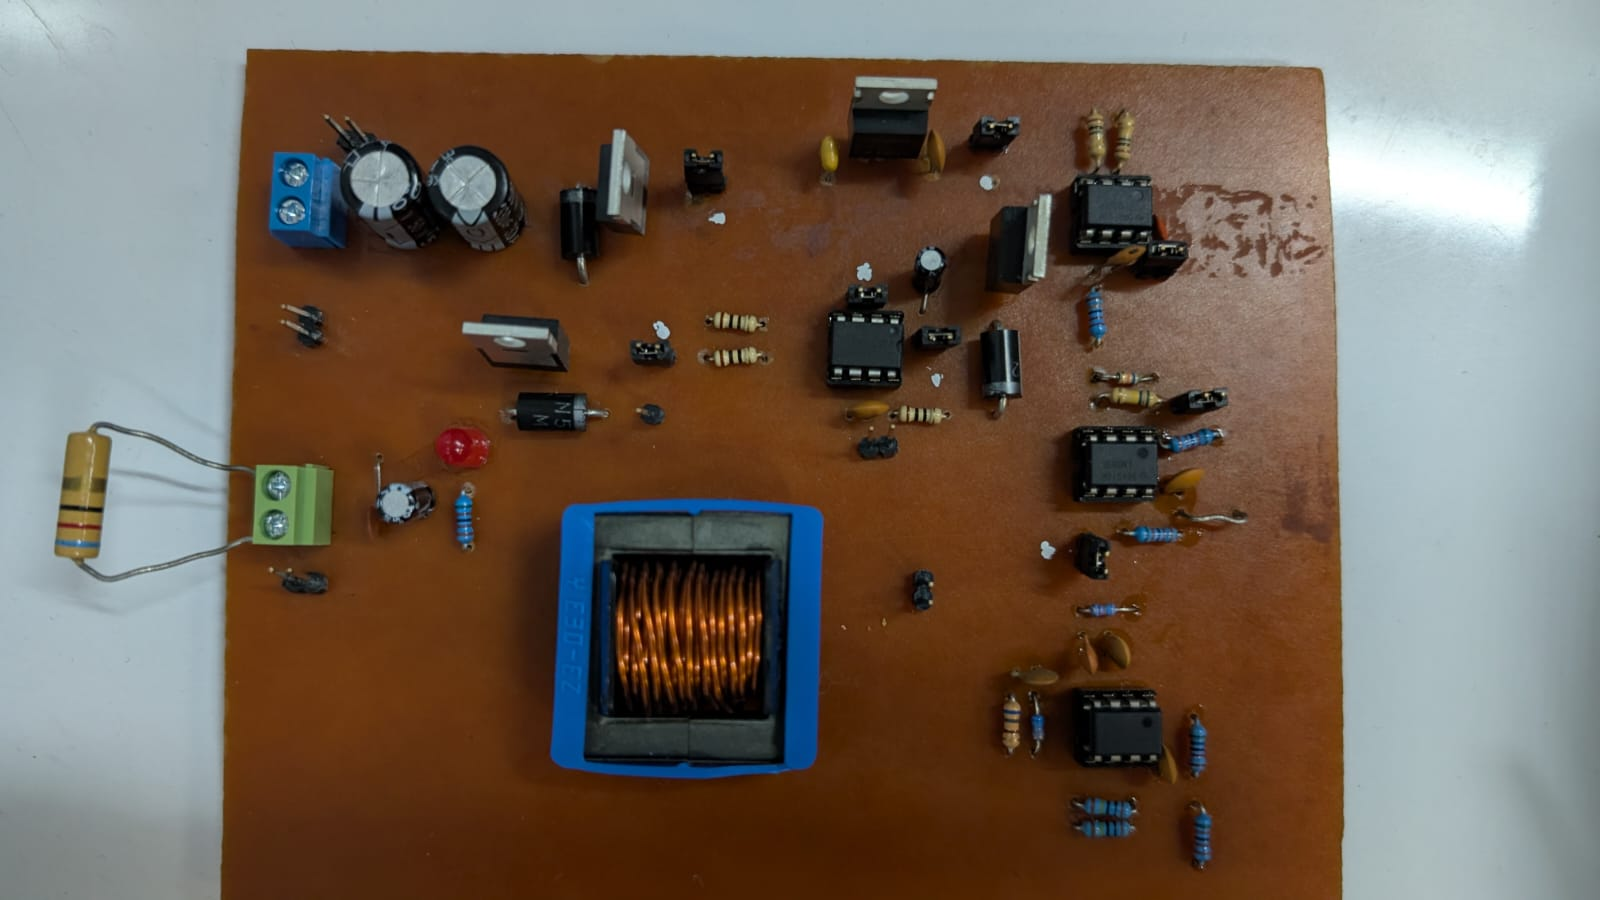
\includegraphics[width=0.9\textwidth]{img/PCB/pcb-final.jpeg}
    \caption{PCB final.}
    \label{fig:PCB_final}
    
\end{figure}

Por último, como se observa en la fig. \ref{fig:PCB_final} se puede apreciar la placa final terminada con los componentes soldados.


\section{Mediciones}
% Incluir gráficos de mediciones.
\subsection{\textit{Gate driver}}

Una vez montado el circuito, se realizó la prueba de funcionamiento del Gate Driver a lazo abierto. El objetivo fue comprobar su correcto funcionamiento a la vez que medir el tiempo muerto, cuando los dos transistores están abiertos.

Para analizar el funcionamiento, se alimentó al Gate Drive con una cuadrad de $\SI{9.4}{\volt}$ pico pico montanda en una contínua de $\SI{4.4}{\volt}$. Se puede apreciar esto en la Figura~\ref{fig:señial entrada gate driver}.

\begin{figure}[H]
    \centering
    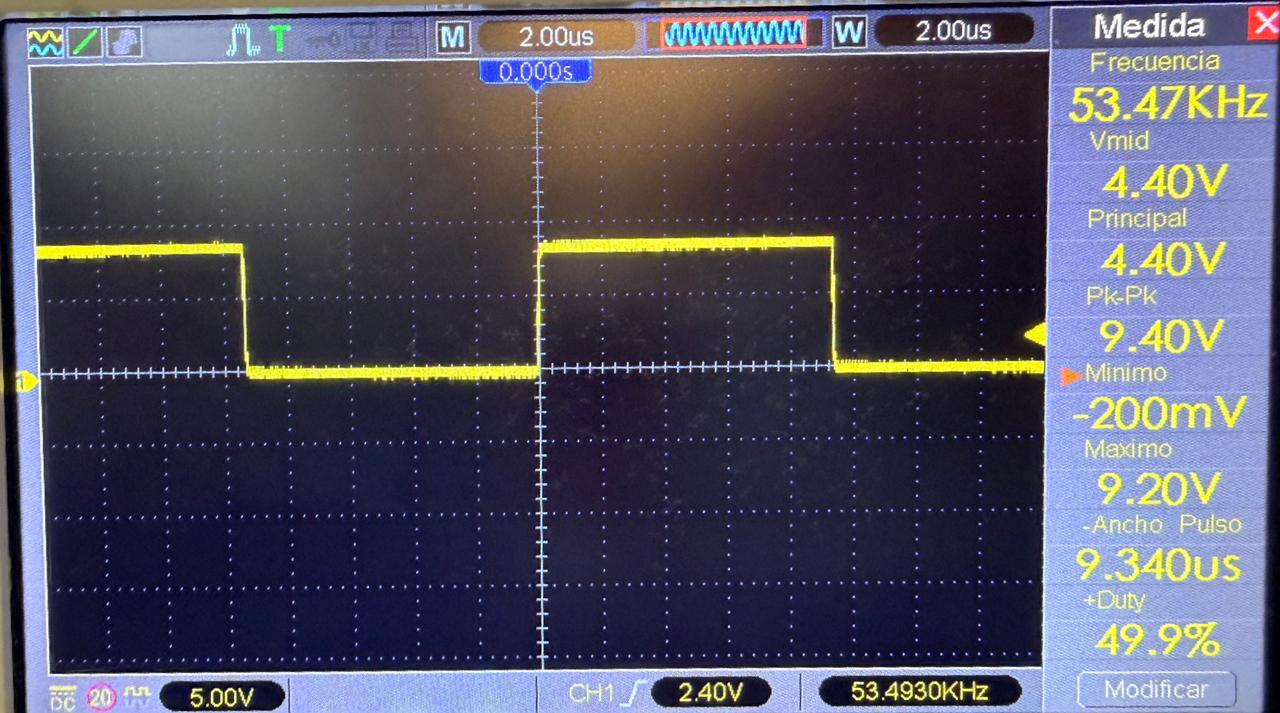
\includegraphics[width=0.8\textwidth]{img/Mediciones imagenes/Entrada GateDriver.png}
    \caption{Señal de entrada del gate Driver.}
    \label{fig:señial entrada gate driver}
\end{figure}

A partir de esta entrada, se obtuvieron, en la Figura~\ref{fig:senial salida gate driver}, las siguientes salidas:

\begin{figure}[H]
    \centering
    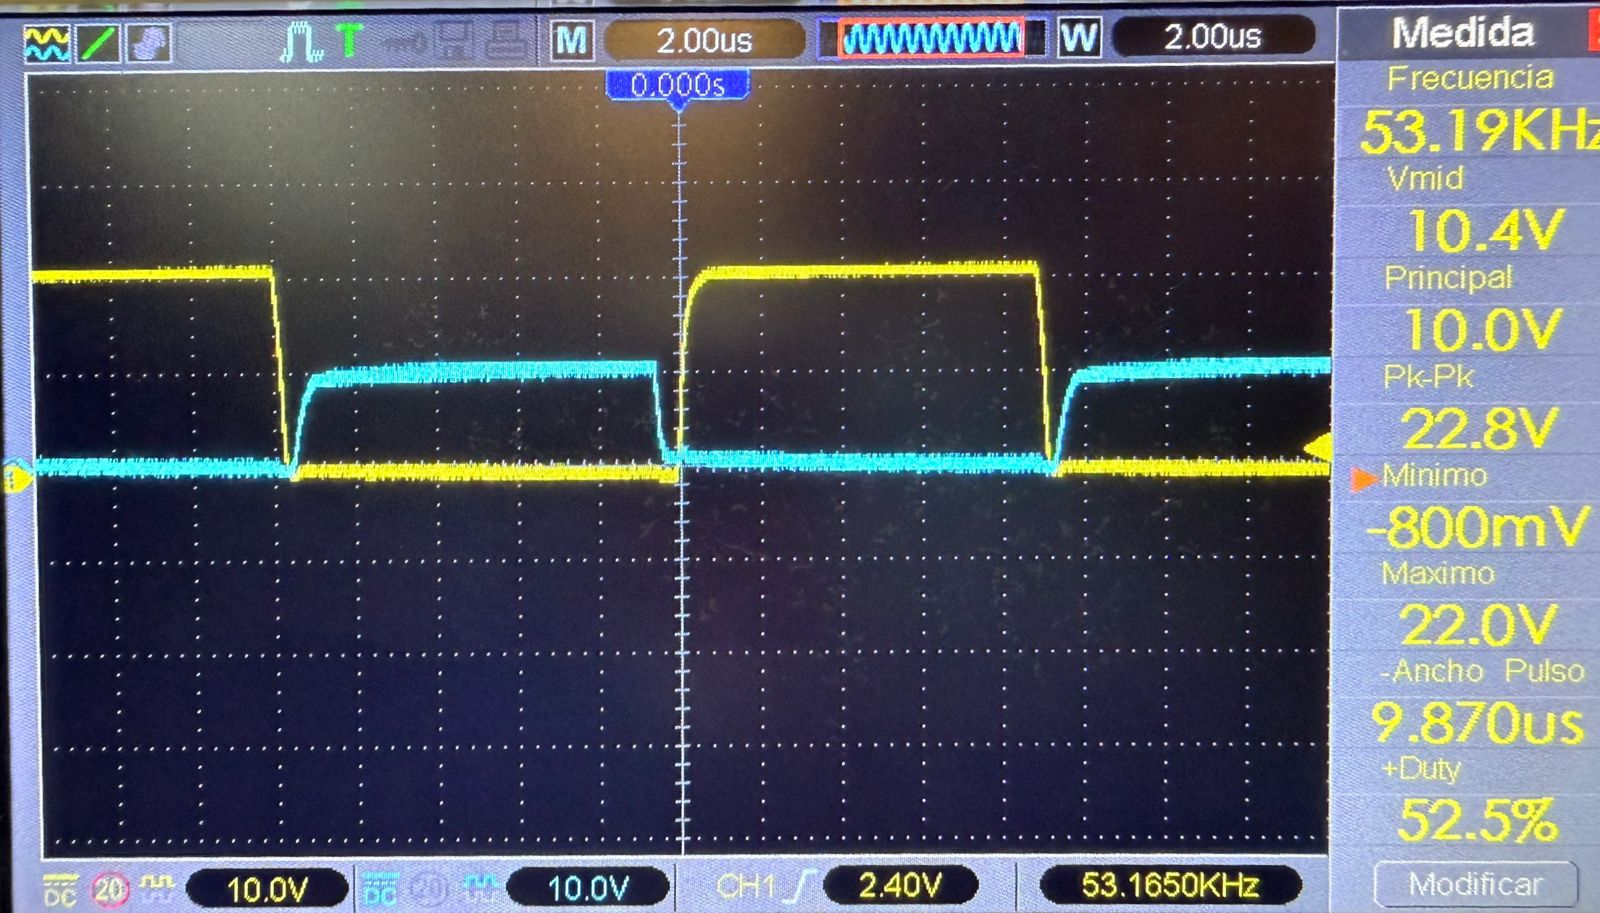
\includegraphics[width=0.9\textwidth]{img/Mediciones imagenes/Salidas GateDriver.jpg}
    \caption{Señales de salida del Gate Driver.}
    \label{fig:senial salida gate driver}
\end{figure}

La diferencia de amplitud entre ambas señales se debe a la forma en que se 
referencian las salidas del Gate Driver. La salida del transistor inferior está 
referida a masa, por lo que conmuta aproximadamente entre $0$ y la tensión de 
alimentación del driver. En cambio, la salida del transistor superior está 
referida al nodo conmutado de la etapa de potencia. Por este motivo, al medirla 
respecto de masa, su tensión incluye tanto la tensión del nodo conmutado como 
la tensión de excitación de compuerta.

Por lo tanto, que una de las señales aparezca con una amplitud mayor no implica 
una amplificación real de la señal de entrada, sino que es consecuencia de medir 
una salida flotante respecto de masa.

Por otro lado, se realizó también la medición del tiempo muerto.

\begin{figure}[H]
    \centering
    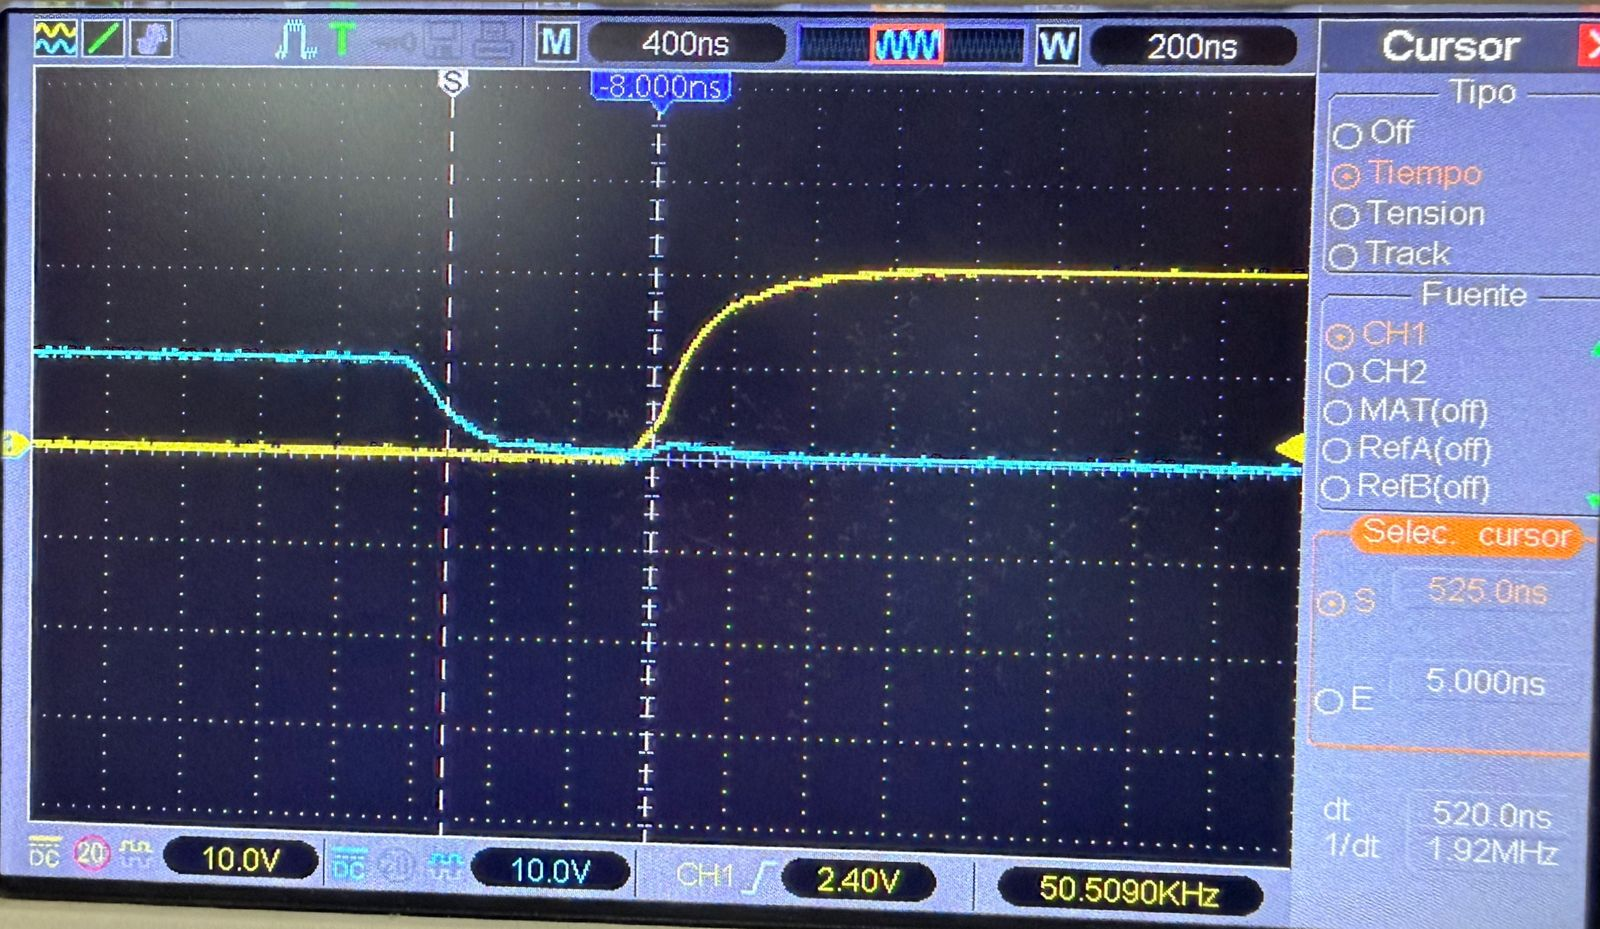
\includegraphics[width=0.9\textwidth]{img/Mediciones imagenes/Tiempo muerto GateDriver.jpg}
    \caption{Tiempo muerto del Gate Driver medido con el osciloscopio.}
    \label{fig:tiempo muerto gate driver}
\end{figure}

En la Figura~\ref{fig:tiempo muerto gate driver} se midió el tiempo muerto del componente en $\SI{520}{\nano\second}$ el cual corresponde al especificado en la hoja de datos del mismo (ver referencias).


\subsection{Conmutación de la \textit{buck}}

Para verificar el funcionamiento de la etapa de potencia se midieron las formas de onda del nodo de conmutación y de la tensión sobre el inductor. Estas mediciones permiten comprobar que las llaves conmutan correctamente y que el inductor alterna entre los intervalos de almacenamiento y entrega de energía propios de un convertidor \textit{buck}.

\begin{figure}[H]
    \centering
    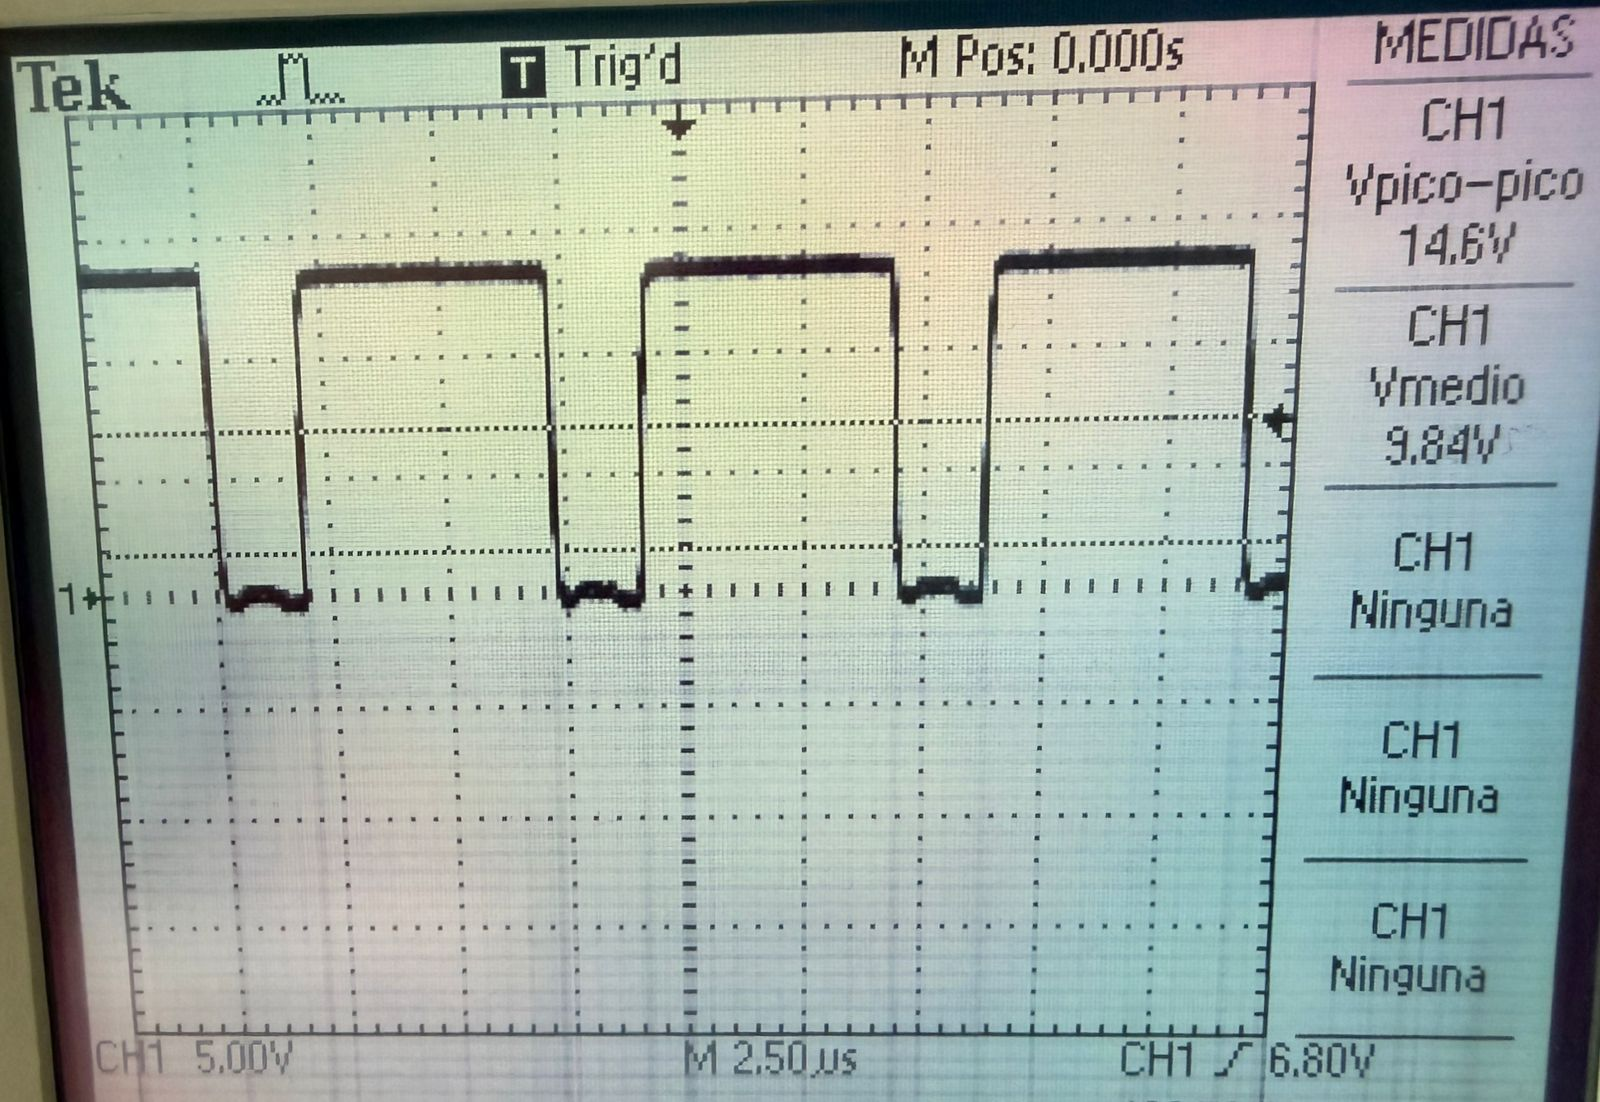
\includegraphics[width=0.8\textwidth]{img/Mediciones imagenes/nodo_conm.jpg}
    \caption{Tensión medida en el nodo de conmutación de la \textit{buck}.}
    \label{fig:nodo_conm}
\end{figure}

En la Figura~\ref{fig:nodo_conm} se observa la tensión del nodo de conmutación. La forma de onda alterna entre un nivel alto, correspondiente al intervalo en que conduce la llave superior, y un nivel bajo, asociado al intervalo de rueda libre. También se aprecian transitorios rápidos en los flancos de conmutación, esperables debido a las capacidades e inductancias parásitas de la etapa de potencia.

\begin{figure}[H]
    \centering
    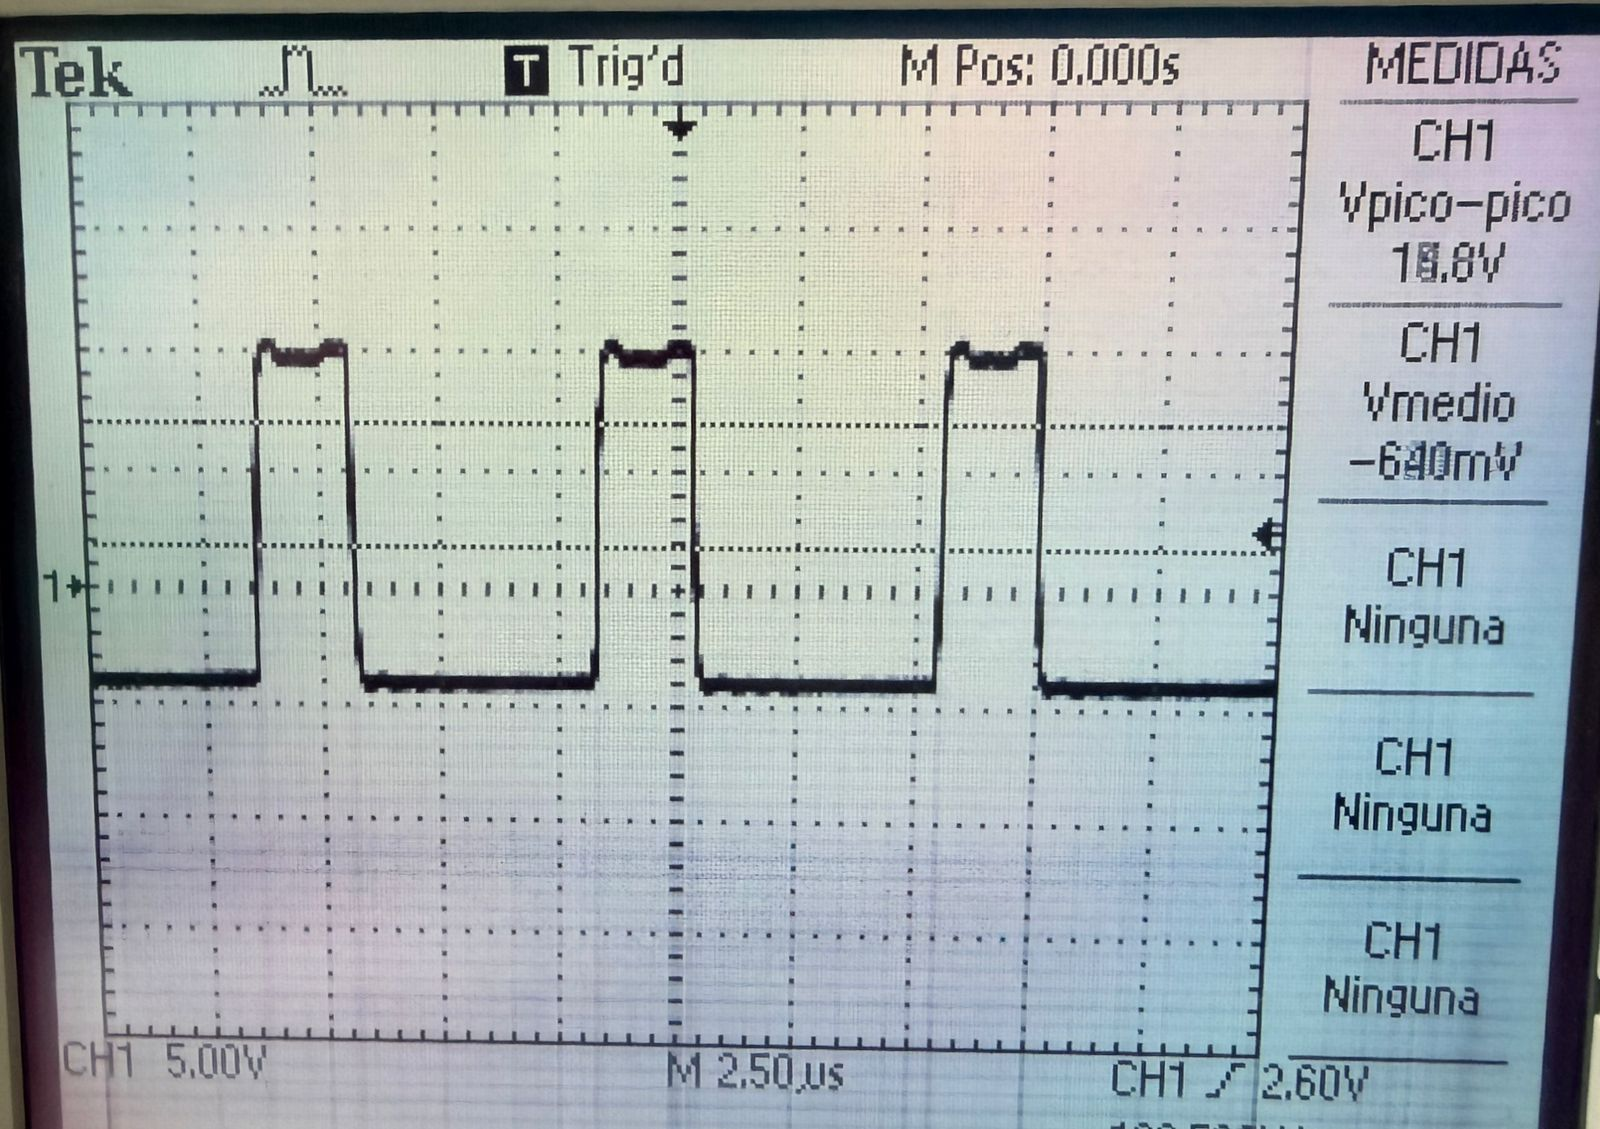
\includegraphics[width=0.8\textwidth]{img/Mediciones imagenes/tension_inductor.jpg}
    \caption{Tensión medida sobre el inductor de la \textit{buck}.}
    \label{fig:tension_inductor}
\end{figure}

En la Figura~\ref{fig:tension_inductor} se muestra la tensión sobre el inductor. Durante el intervalo de conducción de la llave superior, la tensión sobre el inductor es positiva y su corriente aumenta. Durante el intervalo de rueda libre, la tensión cambia de polaridad y la corriente del inductor disminuye. Este comportamiento confirma la transferencia periódica de energía entre la entrada, el inductor y la carga.

\subsection{Eficiencia}
Se midió la eficiencia de la fuente \textit{buck} para diferentes condiciones de carga y tensión de entrada.

\begin{figure}[H]
    \centering
    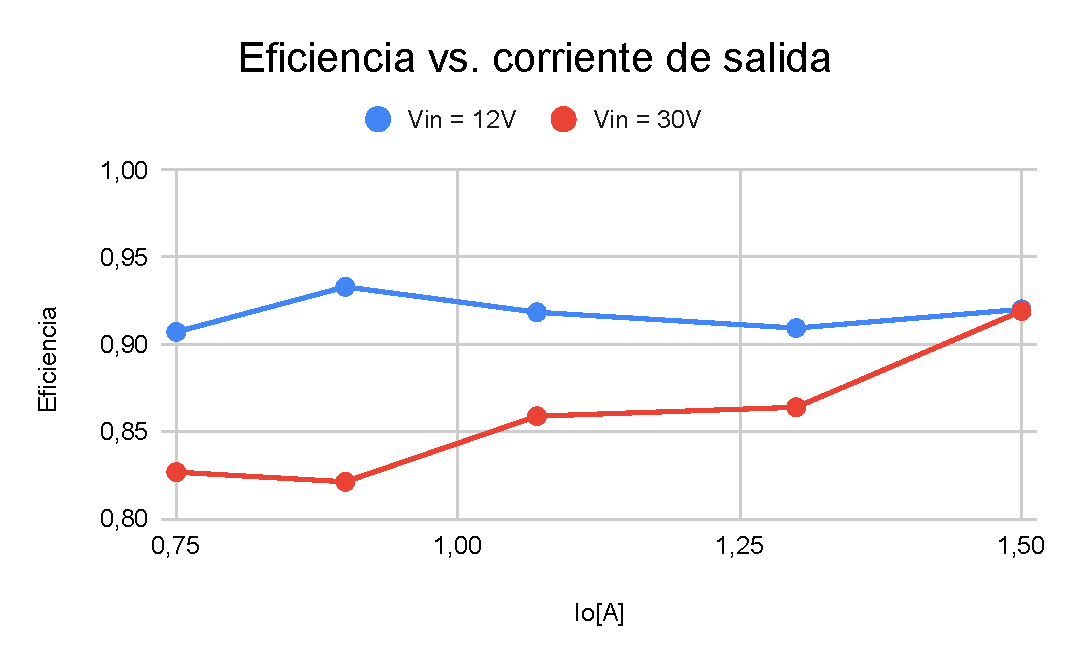
\includegraphics[width=0.8\textwidth]{img/Mediciones imagenes/Eficiencia vs. corriente de salida.pdf}
    \caption{Eficiencia en función de la corriente de salida.}
    \label{fig:ef vs. Io}
\end{figure}

La \autoref{fig:ef vs. Io} muestra la variación de la eficiencia con la corriente de salida para dos tensiones de entrada. Para la curva azul se destaca que en todos los casos la eficiencia fue superior a $90\,$\% y que la misma no varía de forma apreciable con la corriente de salida. Para la curva roja se observa que la eficiencia es menor y que tiende a subir con la corriente de salida. Esto se explica ya que la potencia disipada los reguladores utilizados para alimentar al PWM, a la red de compensación y al \textit{gate driver} aumenta con la tensión de entrada, ya que la caída de tensión en dichos reguladores es mayor. 

\begin{figure}[H]
    \centering
    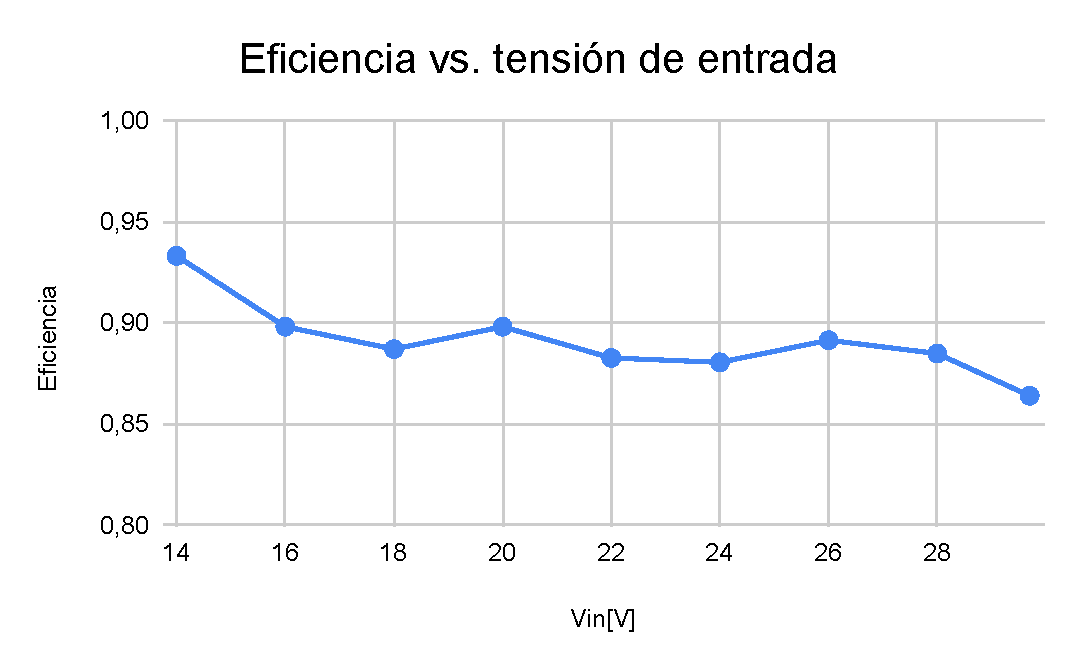
\includegraphics[width=0.8\textwidth]{img/Mediciones imagenes/Eficiencia vs. tensión de entrada.pdf}
    \caption{Eficiencia en función de la tensión de entrada.}
    \label{fig:ef vs. Vin}
\end{figure}

La \autoref{fig:ef vs. Vin} muestra la variación de la eficiencia con la tensión de entrada a una corriente de carga constante $I_o = \SI{0.75}{\ampere}$ . Se destaca que en todos los casos la eficiencia fue superior a $85\,$\% y que la misma decrece ligeramente a mayor tensión de entrada. Esto se debe a que la potencia de salida se mantiene constante (ya que no varía la tensión de salida ni la corriente de salida), mientras que la potencia de entrada aumenta, por lo que el cociente $\eta = \frac{P_O}{P_{IN}}$ disminuye. 

\subsection{Regulación de línea y carga}

\begin{figure}[H]
    \centering
    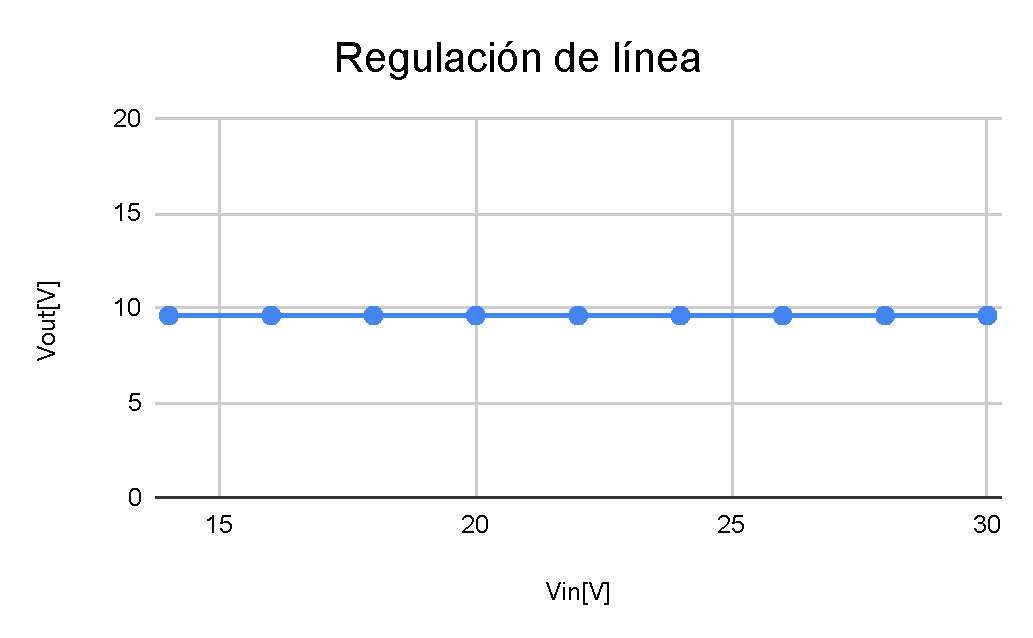
\includegraphics[width=0.8\textwidth]{img/Mediciones imagenes/Regulación de linea.pdf}
    \caption{Regulación de línea.}
    \label{fig:RegLin}
\end{figure}

La \autoref{fig:RegLin} muestra los puntos obtenidos en la medición de la regulación de línea, la cual fue hecha con un osciloscopio ya que la resolución del multímetro resultó insuficiente. Se observó que la tensión de salida apenas varía ante cambios en la tensión de entrada y que esta variación es tan pequeña que no pudo ser apreciada por el multímetro. Se obtuvo entonces $REG_{LIN} = \SI{0.125}{\milli \volt / volt}$.


Por otro lado, para analizar la regulación de carga se midió la tensión de salida $V_o$ 
variando la resistencia de carga $R_L$. Al disminuir esta, la corriente de 
salida aumentó desde $0{.}75\,\text{A}$ hasta $1{.}5\,\text{A}$.

\begin{figure}[H]
    \centering
    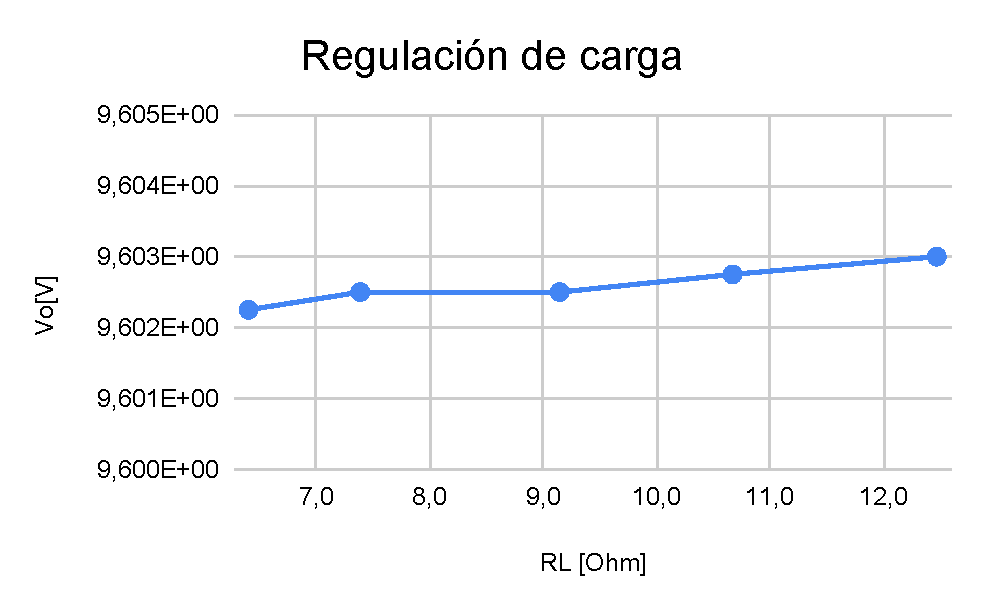
\includegraphics[width=0.8\textwidth]{img/Mediciones imagenes/Regulación de carga.pdf}
    \caption{Regulación de carga}
    \label{fig:RegCar}
\end{figure}

En la fig. \ref{fig:RegCar} se muestra la regulación de carga de la fuente. 
Para esto se midió la tensión de salida \(V_o\) para distintos valores de 
corriente de carga \(I_o\), variando la resistencia \(R_L\).

Se observa que la tensión de salida se mantiene prácticamente constante alrededor 
de \(9{.}6\,\text{V}\), incluso cuando la corriente aumenta desde 
\(0{.}77\,\text{A}\) hasta \(1{.}5\,\text{A}\). Para cuantificar esta variación, 
se calcula la regulación de carga como la pendiente de la recta \(V_o\) en 
función de \(I_o\):

\[
R_{\text{reg}} =
\left|\frac{\Delta V_o}{\Delta I_o}\right|.
\]

Tomando dos puntos de la recta medida,

\[
(I_{o1},V_{o1})=(1{.}3\,\text{A},9{.}6025\,\text{V})
\]

\[
(I_{o2},V_{o2})=(1{.}5\,\text{A},9{.}60225\,\text{V}),
\]

se obtiene

\[
R_{\text{reg}} =
\left|\frac{9{.}60225-9{.}6025}{1{.}5-1{.}3}\right|
=
1{.}25\,\text{m}\Omega.
\]

Este valor es muy bajo, lo que indica que la fuente tiene una buena regulación 
de carga. Es decir, al aumentar la corriente demandada por la carga, la tensión 
de salida prácticamente no cambia.

\subsection{\textit{Ripple} de la tensión de salida}

Como se mencionó en secciones anteriores, el hecho de que el capacitor de salida no se comporte como en la teoría a nuestra frecuencia de operación impidió que el mismo integre eficientemente su corriente, obteniendo un \textit{ripple} lineal en la tensión de salida de la \textit{buck}, tal y como se muestra en la Figura~\ref{fig:ripple_lineal}.

\begin{figure}[H]
    \centering
    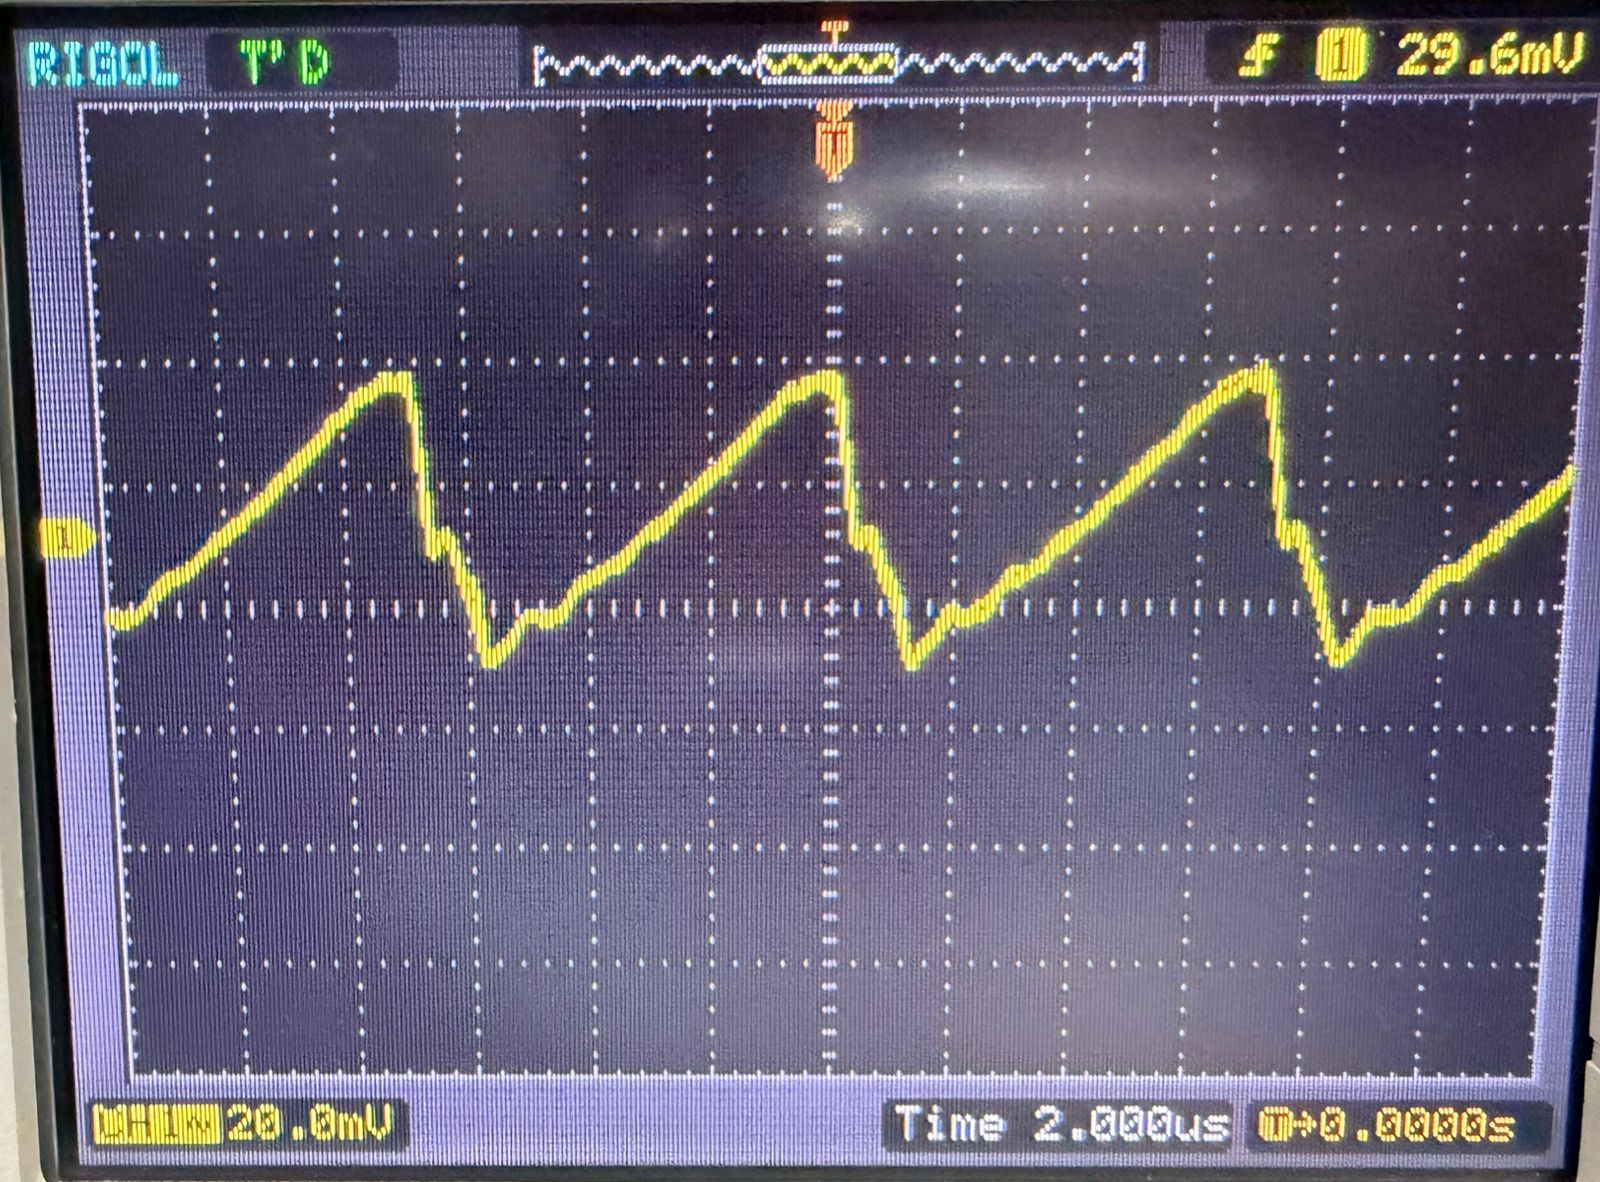
\includegraphics[width=0.8\textwidth]{img/Mediciones imagenes/Salida triangular.jpg}
    \caption{\textit{Ripple} lineal en la tensión de salida de la \textit{buck}.}
    \label{fig:ripple_lineal}
\end{figure}

Para corregir esto se modificó el capacitor de salida de $10\,\upmu$F de una tecnología electrolítica a una cerámica multicapa, la cual no pierde capacitancia a altas frecuencias, permitiendo que el mismo integre correctamente su corriente y obteniendo un \textit{ripple} de tensión cuadrático a la salida de la \textit{buck}, tal y como predice el diseño teórico y como se muestra en la Figura~\ref{fig:ripple_cuad}.

\begin{figure}[H]
    \centering
    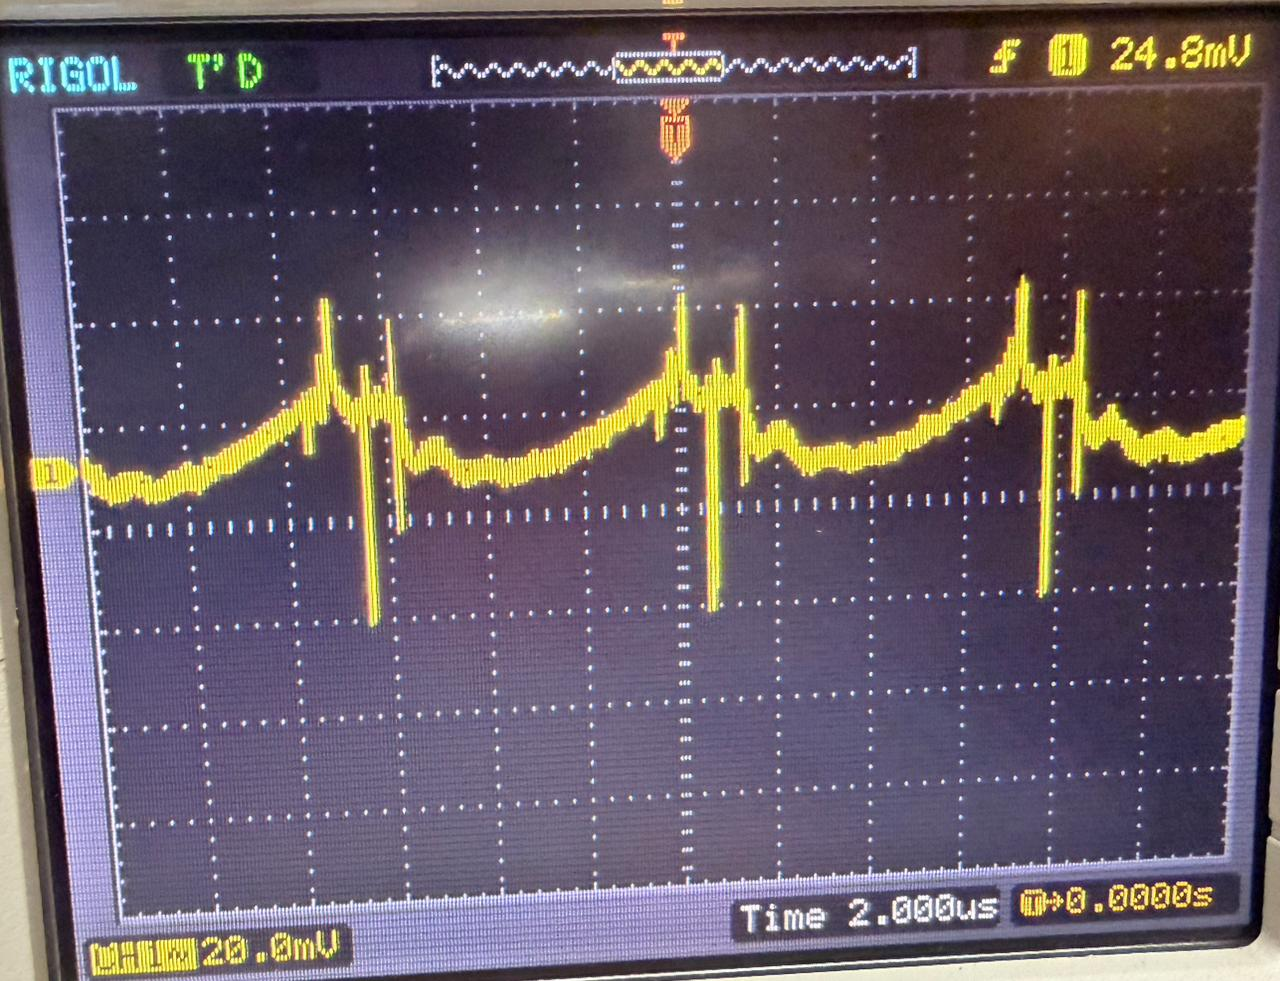
\includegraphics[width=0.8\textwidth]{img/Mediciones imagenes/Salida cuadratica.jpg}
    \caption{\textit{Ripple} cuadrático en la tensión de salida de la \textit{buck}.}
    \label{fig:ripple_cuad}
\end{figure}

\section{Integración final con el LDO}
Como culminación del trabajo realizado durante los últimos cuatro meses, se integró 
finalmente el bloque de la fuente \textit{buck} con el bloque de la LDO 
(ver Fig.~\ref{fig:ldo+buck}). 

\begin{figure}[H]
    \centering
    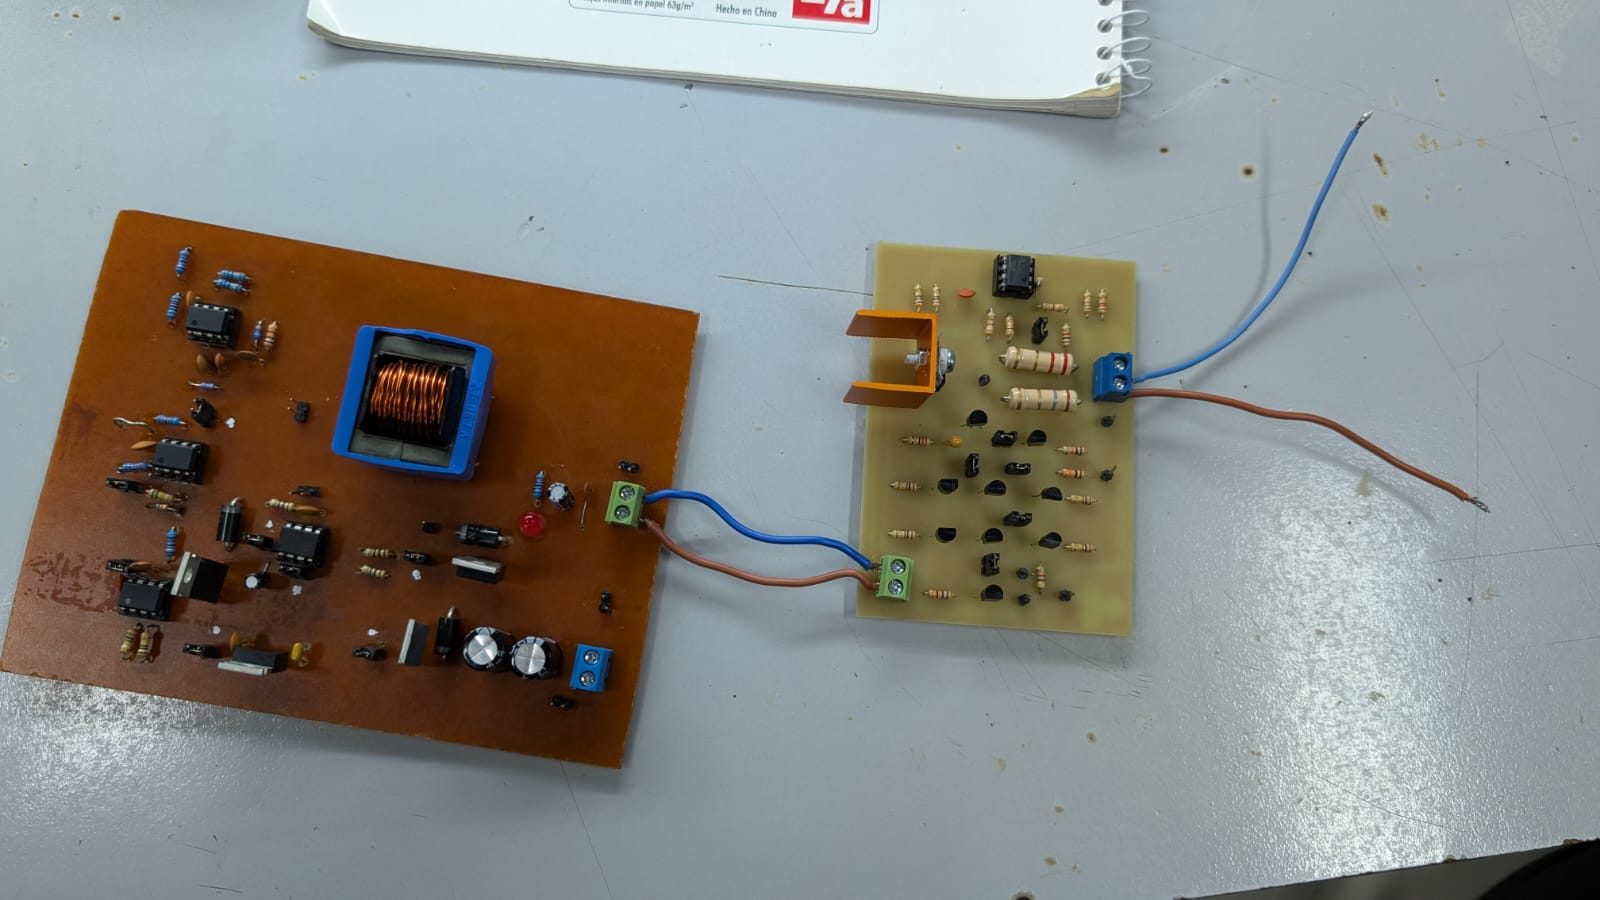
\includegraphics[width=0.65\textwidth]{img/ldo+buck.jpeg}
    \caption{Imagen de la integración de los dos bloques.}
    \label{fig:ldo+buck}
\end{figure}

A partir de esta prueba se verificó el funcionamiento completo del sistema. En 
particular, se observó que la salida de la LDO se mantiene efectivamente 
en \(\SI{5}{\volt}\) para distintos valores de resistencia de carga.

Además, al disminuir la resistencia de carga por debajo de 
\(\SI{3.33}{\ohm}\), se comprobó que se activa correctamente el mecanismo de 
\textit{foldback}, limitando la corriente y reduciendo la tensión de salida. 
Esto confirma que tanto la regulación como la protección de la fuente funcionan 
de acuerdo con lo esperado.

En conclusión, se cumplen con las especificaciones de diseño.



\section{Conclusiones}
A lo largo de este \textit{checkpoint} se complet\'o la integraci\'on, puesta a punto y validaci\'on experimental del convertidor \textit{buck} a lazo cerrado. El trabajo permiti\'o pasar de un dise\~no te\'orico y simulado a una implementaci\'on f\'isica funcional, verificando en cada etapa los bloques principales de la fuente: la etapa de potencia, el circuito de control, el \textit{gate driver}, la red de realimentaci\'on y el PCB final.

En primer lugar, la caracterizaci\'on experimental del inductor confirm\'o que el componente seleccionado era adecuado para la aplicaci\'on. La inductancia medida, de aproximadamente $408{,}7\,\upmu$H, result\'o superior al valor m\'inimo requerido por el dise\~no, mientras que la corriente de saturaci\'on de $4\,$A otorg\'o un margen suficiente frente a las corrientes esperadas durante la operaci\'on normal. Esto permiti\'o asegurar el funcionamiento del convertidor en modo de conducci\'on continua dentro del rango de carga ensayado.

La etapa de control tambi\'en fue ajustada de manera satisfactoria. Las modificaciones realizadas sobre el generador de PWM y el dise\~no de la red de compensaci\'on permitieron estabilizar el sistema a lazo cerrado y mejorar la respuesta frente a perturbaciones. Las simulaciones evidenciaron una reducci\'on de las oscilaciones respecto del sistema sin compensar y una convergencia adecuada de la tensi\'on de salida hacia el valor de referencia, con un margen de fase compatible con una operaci\'on robusta.

En la implementaci\'on pr\'actica se verific\'o el correcto funcionamiento del \textit{gate driver} y se midi\'o un tiempo muerto acorde con el especificado por el fabricante, aspecto fundamental para evitar la conducci\'on simult\'anea de los MOSFET. Adem\'as, la incorporaci\'on de diodos Schottky, capacitores apropiados para la frecuencia de conmutaci\'on y una carga fantasma mejor\'o el comportamiento del circuito durante los transitorios y facilit\'o la realizaci\'on de los ensayos experimentales.

Las mediciones sobre el prototipo confirmaron que la fuente cumple con los objetivos principales del proyecto. Para $V_{in}=12\,$V se obtuvieron eficiencias superiores al $90\%$ dentro del rango de corrientes evaluado, mientras que al variar la tensi\'on de entrada con corriente de carga constante la eficiencia se mantuvo por encima del $85\%$. Asimismo, se observ\'o una buena regulaci\'on de l\'inea y de carga: la tensi\'on de salida present\'o variaciones reducidas, del orden de $10\,$mV al duplicar aproximadamente la corriente de salida.

El desarrollo y fabricaci\'on del PCB permitieron consolidar el dise\~no en una versi\'on compacta y reproducible. Esta etapa puso en evidencia la importancia del trazado de las mallas de corriente, la ubicaci\'on de los capacitores de desacople y salida, y la selecci\'on tecnol\'ogica de los componentes. En particular, el reemplazo del capacitor de salida por uno cer\'amico permiti\'o corregir el comportamiento del \textit{ripple} y acercar la respuesta medida a la prevista te\'oricamente.

En conclusi\'on, se logr\'o dise\~nar, simular, construir y validar experimentalmente una fuente \textit{buck} a lazo cerrado. Si bien durante el proceso aparecieron diferencias entre el modelo ideal y el comportamiento real del circuito, estas fueron identificadas y corregidas mediante ajustes de dise\~no y selecci\'on de componentes. El resultado final presenta una regulaci\'on adecuada, alta eficiencia y estabilidad operativa, por lo que cumple con los requerimientos planteados y constituye una implementaci\'on funcional del sistema propuesto.

\begin{thebibliography}{9}

\bibitem{CosmoFerrites_CF196}
Cosmo Ferrites Ltd.,
\textit{Material Specifications CF196},
Material Data Sheet,
4 August 2017.

\bibitem{CosmoFerrites_EE3007}
Cosmo Ferrites Ltd.,
\textit{Product Data Sheet: Core EE3007},
Product Data Sheet.

\bibitem{Zhang2015}
H. J. Zhang,
``Modelado y diseño de compensación de lazo en fuentes de alimentación conmutadas. Parte 1ª'',
\textit{Revista Española de Electrónica (REE)},
n.º 96, pp. 96--101, octubre de 2015.
Artículo cedido por Linear Technology.

\bibitem{IR2104_datasheet}
International Rectifier,
\textit{IR2104(S) \& IR2104S(PbF) Half-Bridge Driver Datasheet},
Data Sheet No. PD60046-S, Abril 2004.

\bibitem{LM2576_datasheet}
Texas Instruments,
\emph{LM2576, LM2576HV SIMPLE SWITCHER (R) 3-A Step-Down Voltage Regulator Datasheet},
Document No.~SNVS107G,
Revision~G, March~2023.

\bibitem{Vishay_030031AS}
Vishay BCcomponents,
\textit{030/031 AS Aluminum Electrolytic Capacitors, Axial Standard},
Document Number~28327,
Revision: 16 September 2016.

\end{thebibliography}

\end{document}